\documentclass[10pt,a4paper,oneside]{article}
\usepackage[brazil]{babel}
\usepackage[utf8]{inputenc}
\usepackage{amsmath}
\usepackage{amsfonts}
\usepackage{amssymb}
\usepackage[left=3cm,right=3cm,top=2cm,bottom=2cm]{geometry}


% Floats.
\usepackage{placeins}

% Captions
\usepackage{caption}
\usepackage{capt-of}

\usepackage{xspace}
\usepackage{graphicx}

\newcommand{\arat}{Aratibutantã\xspace}
\newcommand{\baep}{Baependinha\xspace}
\newcommand{\itam}{Itamaracanã\xspace}
\newcommand{\jaqu}{Jaquereçaba\xspace}
\newcommand{\para}{Paranapitanga\xspace}

\newcommand{\adm}{Administração\xspace}
\newcommand{\comp}{Computação e Matemática\xspace}
\newcommand{\edu}{Educacional\xspace}
\newcommand{\eng}{Engenharia e Produção\xspace}
\newcommand{\hum}{Humanidades\xspace}
\newcommand{\jur}{Jurídica e Contábil\xspace}

% Tabelas.
\usepackage{multirow}
\usepackage{booktabs}
\newcommand{\specialcell}[3][c]
{\begin{tabular}[#1]{@{}#2@{}}#3\end{tabular}}

\author{%
	Alexis A. Huf, %
	Alyson D. Pereira, %
	Bruno C. N. Oliveira,\\%
	Eliza Gomes, %
	Pedro H. Penna
	}

\title{Lista de Exercício I - Grupo 6}


\begin{document}

\maketitle

\section*{Parte 1: Pré-Análise de Dados}

\paragraph{Questão 01}

A Tabela \ref{table: dados perdidos} apresenta a quantidade de dados perdidos (aqueles que não puderam ser recuperados por não estarem preenchidos) e seus respectivos percentuais em relação a cada variável analisada na base de dados em estudo. Foi observado um total de 106 dados perdidos para todas as variáveis, o que representa apenas $2.12\%$ do total. Pode-se considerar, portanto, como aceitável, uma vez que está abaixo dos $5\%$ definidos como percentual aceitável de dados perdidos.



%
% Dúvidas:
%   Devemos detalhar quis os erros (ex: Arábia, Araba)?
%
\paragraph{Questão 02}

A Tabela \ref{table: dados errados} resume os erros de coleta e seus respectivos percentuais na base de dados em estudo. Além de ausência de informação (conforme já mencionado na \textbf{Questão 01}), foram evidenciados erros de ortografia, digitação e formatação (ex: espaços em branco excedentes). 

As Tabelas \ref{table: erros-regiao}, \ref{table: erros-area}, \ref{table: erros-pagamento} e \ref{table: erros-opiniao} apresentam os erros observados para as variáveis qualitativas \textit{Região}, \textit{Área}, \textit{Pagamento} e \textit{Opinião}, respectivamente.
Para as variáveis quantitativas \textit{Renda} e \textit{Idade}, não foram observados erros na base de dados, isto é, valores infactíveis (ex: \textit{Renda} não positiva e \textit{Idade} inferior a 17 ou superior a 100 anos).

Para evitar que erros de ortografia e formatação sejam cometidos nas variáveis qualitativas, pode-se utilizar um formulário de múltipla escolha de modo a evitar que as informações sejam preenchidas de maneira textual. Já para as variáveis quantitativas, no caso de um formulário eletrônico, limites inferiores e superiores de valores válidos poderiam ser checado previamente à submissão da observação. Por outro lado, quanto aos dados perdidos que não foram preenchidos, é possível criar opções de modo que as pessoas possam informar explicitamente se não sabem ou, ainda, se não desejam responder. Desse modo, nenhuma informação seria ficaria perdida ou sem preenchimento. Ademais, é possível também aplicar um teste do questionário a um grupo menor de pessoas com o objetivo de testá-lo e verificar a sua adequação, para, posteriormente, aplicá-lo a um grupo maior. Assim, problemas de entendimento podem ser resolvidos nesta fase de teste, tendendo a reduzir o percentual de erros ou informações faltantes.

\begin{figure}[h]
\begin{minipage}{0.49\textwidth}
\centering
\captionof{table}{Dados perdidos na base de dados.}
\label{table: dados perdidos}
\vspace{0.5em}
\begin{tabular}{l r r}
	\toprule
	\textbf{Variável} & \textbf{\specialcell{c}{Dados\\Perdidos}} & \textbf{\specialcell{c}{Perdas\\Percentuais}} \\
	\midrule
	Área              & $21$            & $0,42\%$          \\
	Idade             & $13$            & $0,26\%$          \\
	Opinião           & $19$            & $0,38\%$          \\
	Pagamento         & $18$            & $0,36\%$          \\
	Região            & $21$            & $0,42\%$          \\
	Renda             & $14$            & $0,28\%$          \\
	\bottomrule
\end{tabular}
\end{minipage}
%
\begin{minipage}{0.49\textwidth}
\centering
\captionof{table}{Erros na base de dados.}
\label{table: dados errados}
\vspace{0.5em}
\begin{tabular}{l r r}
	\toprule
	\textbf{Variável} & \textbf{\specialcell{c}{Dados\\Errados}} & \textbf{\specialcell{c}{Erros\\Percentuais}} \\
	\midrule
	Área              & $114$                                    & $2,28\%$          \\
	Idade             & $0$                                      & $0,00\%$          \\
	Opinião           & $123$                                    & $2,46\%$          \\
	Pagamento         & $132$                                    & $2,64\%$          \\
	Região            & $135$                                    & $2,71\%$          \\
	Renda             & $0$                                      & $0,00\%$          \\
	\bottomrule
\end{tabular}
\end{minipage}
\end{figure}

\begin{table}[!h]
\centering
\begin{minipage}[t]{0.49\textwidth}
\caption{Erros para a variável \textit{Região}.}
\vspace{0.5em}
\label{table: erros-regiao}
\begin{tabular}{l r r}
	\toprule
	\textbf{Erro} & \textbf{Absoluto}  & \textbf{Percentual} \\
	\midrule
	Arati      & 6  & $0.12\%$ \\
	Aratib     & 12 & $0.24\%$ \\
	Aratibu    & 5  & $0.10\%$ \\
	Aratibut   & 12 & $0.24\%$ \\
	Baepe      & 17 & $0.34\%$ \\
	Baepen     & 18 & $0.36\%$ \\
	Baepend    & 12 & $0.24\%$ \\
	Baependi   & 9  & $0.18\%$ \\
	Itama      & 5  & $0.10\%$ \\
	Itamar     & 6  & $0.12\%$ \\
	Itamara    & 3  & $0.06\%$ \\
	Itamarac   & 7  & $0.14\%$ \\
	Jaque      & 5  & $0.10\%$ \\
	Jaquer     & 10 & $0.20\%$ \\
	Jaquere    & 5  & $0.10\%$ \\
	Jaquereç   & 3  & $0.06\%$ \\
	\midrule
	\textbf{Total de erros}  & 135  & $2.71\%$ \\	
	\bottomrule
\end{tabular}
\end{minipage}
%
\begin{minipage}[t]{0.49\textwidth}
\caption{Erros para a variável \textit{Área}.}
\vspace{0.5em}
\label{table: erros-area}
\begin{tabular}{l r r}
	\toprule
	\textbf{Erro} & \textbf{Absoluto}  & \textbf{Percentual} \\
	\midrule
	Admin      & 3   & $0.06\%$ \\
	Admini 	   & 3   & $0.06\%$ \\
	Adminis    & 2   & $0.04\%$ \\
	Administ   & 5   & $0.10\%$ \\
	Compu      & 1   & $0.02\%$ \\
	Comput     & 2   & $0.04\%$ \\
	Computa    & 2   & $0.04\%$ \\
	Computaç   & 1   & $0.02\%$ \\
	Educa      & 2   & $0.04\%$ \\
	Educac     & 2   & $0.04\%$ \\
	Educaci    & 1   & $0.02\%$ \\
	Educacio   & 1   & $0.02\%$ \\
	Engen      & 15  & $0.30\%$ \\
	Engenh     & 9   & $0.18\%$ \\
	Engenha    & 8   & $0.16\%$ \\
	Engenhar   & 14  & $0.28\%$ \\
	Human      & 3   & $0.06\%$ \\
	Humani     & 3   & $0.06\%$ \\
	Humanid    & 4   & $0.08\%$ \\
	Humanida   & 5   & $0.10\%$ \\
	Juríd      & 3   & $0.06\%$ \\
	Jurídi     & 7   & $0.14\%$ \\
	Jurídic    & 11  & $0.22\%$ \\
	Jurídica   & 7   & $0.14\%$ \\	
	\midrule
	\textbf{Total de erros}  & 114  & $2.28\%$ \\	
	\bottomrule
\end{tabular}
\end{minipage}
\end{table}

\begin{table}[!h]
\centering
\begin{minipage}[t]{0.49\textwidth}
\caption{Erros para a variável \textit{Pagamento}.}
\vspace{0.5em}
\label{table: erros-pagamento}
\begin{tabular}{l r r}
	\toprule
	\textbf{Erro} & \textbf{Absoluto}  & \textbf{Percentual} \\
	\midrule
	Auxíl     		& 3   & $0.06\%$ \\
	Auxíli 	  		& 2   & $0.04\%$ \\
	Auxílio    	 	& 2   & $0.04\%$ \\
	Auxílio \textit{(espaço)}   	& 1   & $0.02\%$ \\
	Bolsa      	 	& 3   & $0.06\%$ \\
	Bolsas     	 	& 1   & $0.02\%$ \\
	Bolsas d   	 	& 5   & $0.10\%$ \\
	Finan      	 	& 15  & $0.30\%$ \\
	Financ     	 	& 13  & $0.26\%$ \\
	Financi    	 	& 19  & $0.38\%$ \\
	Financia   	 	& 13  & $0.26\%$ \\
	Incen      	 	& 8   & $0.16\%$ \\
	Incent     	 	& 11  & $0.22\%$ \\
	Incenti    	 	& 11  & $0.22\%$ \\
	Incentiv   	 	& 10  & $0.20\%$ \\
	Recur      	 	& 4   & $0.08\%$ \\
	Recurs     	 	& 4   & $0.08\%$ \\
	Recurso    	 	& 5   & $0.10\%$ \\
	Recursos   	 	& 2   & $0.04\%$ \\	
	\midrule
	\textbf{Total de erros}  & 132  & $2.64\%$ \\	
	\bottomrule
\end{tabular}
\end{minipage}
%
\begin{minipage}[t]{0.49\textwidth}
\caption{Erros para a variável \textit{Opinião}.}
\vspace{0.5em}
\label{table: erros-opiniao}
\begin{tabular}{l r r}
	\toprule
	\textbf{Erro} & \textbf{Absoluto}  & \textbf{Percentual} \\
	\midrule
	Indifer    & 14  & $0.28\%$ \\
	Indifere   & 16  & $0.32\%$ \\
	Insatis    & 7   & $0.14\%$ \\
	Insatisf   & 10  & $0.20\%$ \\
	Muito i    & 3   & $0.06\%$ \\
	Muito in   & 5   & $0.10\%$ \\
	Muito s    & 22  & $0.44\%$ \\
	Muito sa   & 28  & $0.56\%$ \\
	Satisfe    & 10  & $0.20\%$ \\
	Satisfei   & 8   & $0.16\%$ \\	
	\midrule
	\textbf{Total de erros}  & 123  & $2.46\%$ \\	
	\bottomrule
\end{tabular}
\end{minipage}
\end{table}


\begin{table}[!h]
\centering

\end{table}

\FloatBarrier

\clearpage
\section*{Parte 2: Análise Individual das Variáveis}

Nessa segunda parte é apresentada uma análise individual das variáveis da amostra. Para o estudo das variáveis qualitativas (\textit{Região}, \textit{Área}, \textit{Pagamento} e \textit{Opinião}) utilizou-se a tabela de frequências. Já para análise das variáveis quantitativas, fez-se o uso de medidas de síntese e histogramas.

\subsection*{Variável \textit{Região}}

A tabela frequências para a variável \textit{Região} é apresentada na Tabela \ref{table: frequencias regiao}. A análise indica que as regiões com menor e maior número de alunos são as regiões \textit{\para} e \textit{\baep}, respectivamente. Já as demais regiões apresentam um corpo discente que varia de $10,77\%$ a $23,80\%$.

\begin{table}[h]
\small
\centering
\caption{Frequências para a variável \textit{Região}}
\label{table: frequencias regiao}
\vspace{0.5em}
\begin{tabular}{l r r}
	\toprule
	\textbf{Região} & \textbf{Ocorrências} & \textbf{Frequência} \\
	\midrule
	\arat           & $1185$               & $23,80\%$           \\
	\baep           & $2294$               & $46,07\%$           \\
	\itam           & $843$                & $16,93\%$           \\
	\jaqu           & $536$                & $10,77\%$           \\
	\para           & $121$                & $2,43\%$            \\
	\bottomrule
\end{tabular}
\end{table}

\subsection*{Variável \textit{Área}}

A tabela de frequências para a variável \textit{Área} é apresentada na Tabela \ref{table: frequencias area}. O perfil da TYU modificou-se. A análise indica que a área com o maior contingente de alunos é \textit{\eng}, na amostra atual.

\begin{table}[h]
\small
\centering
\caption{Frequências para a variável \textit{Área}}
\label{table: frequencias area}
\vspace{0.5em}
\begin{tabular}{l r r}
	\toprule
	\textbf{Área} & \textbf{Ocorrências} & \textbf{Frequência} \\
	\midrule
	\adm            & $592$                & $11,89\%$           \\
	\comp           & $296$                & $5,94\%$            \\
	\edu            & $338$                & $6,79\%$            \\
	\eng            & $1741$               & $34,97\%$           \\
	\hum            & $503$                & $10,10\%$           \\
	\jur            & $1509$               & $30,31\%$           \\
	\bottomrule
\end{tabular}
\end{table}

\subsection*{Variável \textit{Pagamento}}

A tabela de frequências para a variável \textit{Pagamento} á apresentada na Tabela \ref{table: frequencias pagamento}. A análise indica que os recursos usados para pagar as mensalidades do curso são oriundos, em sua maioria, de \textit{Financiamento Bancário} ($43,98\%$) seguido por \textit{Incentivos Federais} ($29,06\%$), somando um total de $73,04\%$. Portanto, cortes no orçamento federal de Pindorama não afetarão a fonte de recursos primária para pagamentos de mensalidades na TYU.

\begin{table}[h]
\small
\centering
\caption{Frequências para a variável \textit{Pagamento}}
\label{table: frequencias pagamento}
\vspace{0.5em}
\begin{tabular}{l r r}
	\toprule
	\textbf{Pagamento}     & \textbf{Ocorrências} & \textbf{Frequência} \\
	\midrule
	Auxilio Familiar       & $257$                & $5,16\%$            \\
	Bolsas                 & $328$                & $6,58\%$            \\
	Financiamento Bancário & $2191$               & $43,98\%$           \\
	Incentivos Federais    & $1448$               & $29,06\%$           \\
	Recursos Próprios      & $758$                & $15,21\%$           \\
	\bottomrule
\end{tabular}
\end{table}

\subsection*{Variável \textit{Opinião}}

A tabela de frequências para a variável \textit{Opinião} é apresentada na Tabela \ref{table: frequencias opiniao}. A análise indica que opinião predominante na amostra é \textit{Muito Satisfeito} e que o grupo de alunos que mencionaram estarem \textit{Muito satisfeito} ou \textit{Satisfeito} totaliza $55,29\%$. Portanto, pode-se considerar que a maioria dos alunos da TYU estão satisfeitos com a EAD.

\begin{table}[h]
\small
\centering
\caption{Frequências para a variável \textit{Opinião}}
\label{table: frequencias opiniao}
\vspace{0.5em}
\begin{tabular}{l r r}
	\toprule
	\textbf{Pagamento}     & \textbf{Ocorrências} & \textbf{Frequência} \\
	\midrule
	Muito Insatisfeito     & $472$                & $9,48\%$            \\
	Insatisfeito           & $749$                & $15,04\%$           \\
	Indiferente            & $1006$               & $20,20\%$           \\
	Satisfeito             & $1035$               & $20,78\%$           \\
	Muito Satisfeito       & $1719$               & $34,51\%$           \\
	\bottomrule
\end{tabular}
\end{table}

\subsection*{Variável \textit{Renda}}

Medidas de síntese para a variável \textit{Renda} são apresentadas na Tabela \ref{table: medidas sintese renda}. Além disso, um histograma da variável renda é apresentado na Figura \ref{figure: histograma renda}. Vale ressaltar que, para fins de estudo, aplicou-se uma transformação nessa variável, utilizando como fator multiplicativo o valor de $R\$880$ (referência salarial em Pindorama). 

A análise indica que pelo menos três três quartos dos alunos de EAD da TYU ainda mantém renda familiar inferior a $R\$2450,00$, uma vez que o quartil superior da amostra para essa variável é de $R$\$$2402,40$. Além disso constata-se que a distribuição da variável segue uma curva leptocúrtica (curtose $> 0$), possui assimetria à direita (assimetria $> 0$) e dispersão de $76\%$ em relação à média. Com relação aos valores discrepantes, observa-se que o conjunto de dados analisados e disponíveis na base de dados contempla $296$ valores de renda acima de R\$ $4224,00$.

\begin{figure}[h]
\centering
\begin{minipage}{0.52\textwidth}
\centering
\small
\captionof{table}{Medidas de síntese para variável \textit{Renda}.}
\vspace{0.5em}
\label{table: medidas sintese renda}
\begin{tabular}{l r}
	\toprule
	\textbf{Medida}               & \textbf{Renda}    \\
	\midrule
	Média                         &  R\$ $2056,05$    \\
	Moda                          &  R\$ $906,40$     \\
	Mediana                       &  R\$ $1628,00$    \\
	Variância                     &  R\$ $2449929,23$ \\
	Desvio Padrão                 &  R\$ $1565.38$    \\
	Coeficiente de Variação       &  $76\%$           \\
	Assimetria                    &  $9.94$           \\
	Curtose                       &  $253.91$         \\
	Mínimo                        &  R\$ $880.00$     \\
	Máximo                        &  R\$ $53504.00$   \\
	Quartil Inferior (Qi)         &  R\$ $1188.00$    \\
	Quartil Superior (Qs)         &  R\$ $2402.40$    \\
	Diferença Interquartil        &  R\$ $1214.40$    \\
	$Qi-1.5x(Qs-Qi)$              &  R\$ ${-633.60}$  \\
	$Qs+1.5x(Qs-Qi)$              &  R\$ $4224.00$    \\
	Dados Totais                  &  $5000$           \\
	Dados Válidos                 &  $4986$           \\
	Dados Perdidos                &  $14$             \\
	Dados Discrepantes            &  $296$            \\
	\bottomrule
\end{tabular}
\end{minipage}
%
\begin{minipage}{0.46\textwidth}
	\centering
	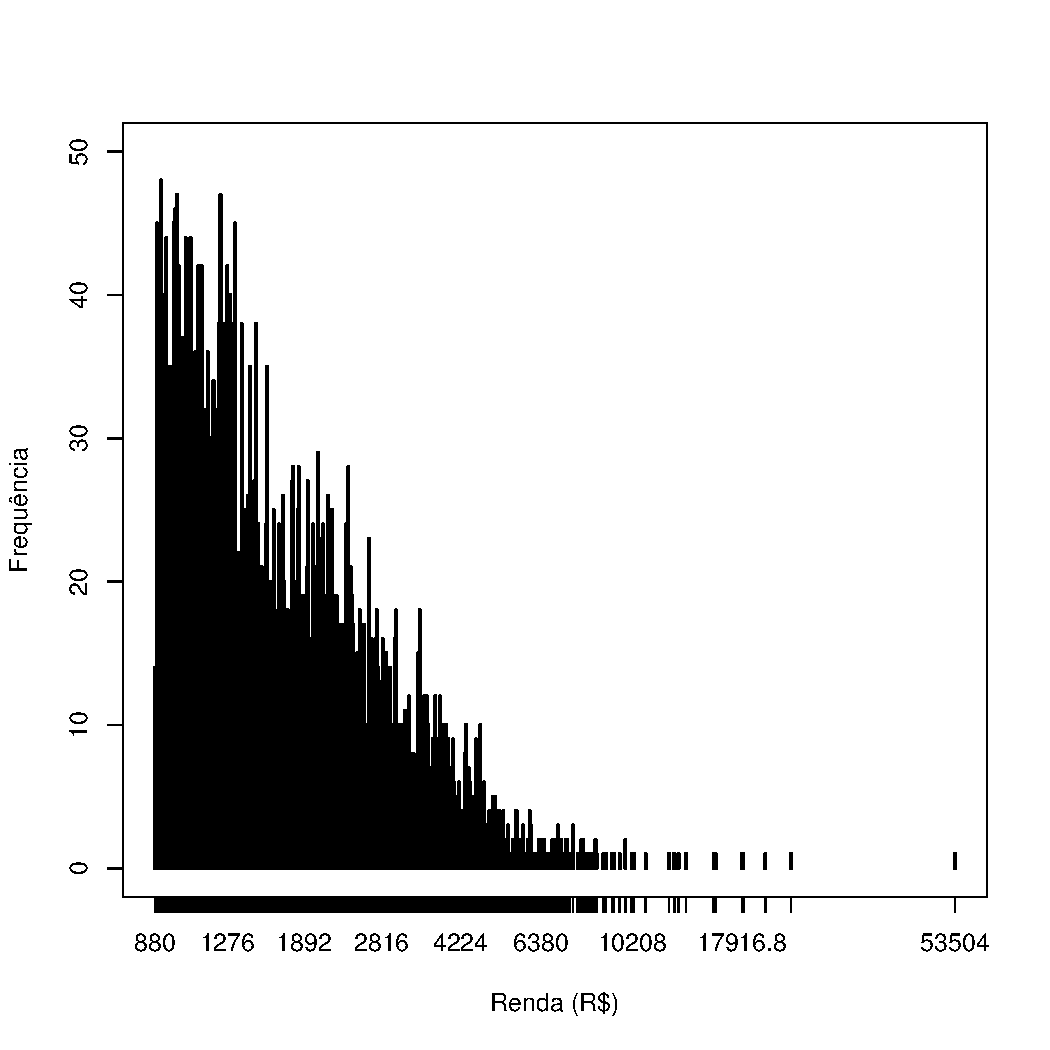
\includegraphics[width=\linewidth]{plots/histograma-renda}
	\captionof{figure}{Histograma da varável \textit{Renda}.}
	\label{figure: histograma renda}
\end{minipage}
\end{figure}

\clearpage
\subsection*{Variável \textit{Idade}}

Medidas de síntese para a variável \textit{Renda} são apresentadas na Tabela \ref{table: medidas sintese idade}. Além disso, um histograma da variável renda é apresentado na Figura \ref{figure: histograma idade}.

A análise indica que a maioria dos alunos de EAD na TYU possuem mais de $30$ anos. Essa conclusão pode ser tomada com base mediana, que assume valor $32$ anos. Mais especificamente, a proporção de alunos com mais de 30 anos na amostra é de $61,4\%$. Fazendo uma comparação com o perfil antigo, pode-se afirmar que o perfil dos alunos mudou, agora a maioria dos alunos são dois anos mais velhos, de $30$ para $32$ anos.

Fazendo uma análise mais detalhada da variável em estudo, percebe-se que ela segue uma distribuição com curtose leptocúrtica (curtose $> 0$), assimetria positiva (assimetria $> 0$) e dispersão de $18\%$ em relação à média. Além disso, podemos observar que pelo quartil inferior e superior, que $50\%$  dos alunos possuem de $29$ a $35$ anos. Vale observar, que dos $98$ valores discrepantes na amostra, a maioria ($69$ observações) encontram-se superiores a $44$ anos.

\begin{figure}[h]
\centering
\begin{minipage}{0.52\textwidth}
\centering
\small
\captionof{table}{Medidas de síntese para variável \textit{Idade}.}
\vspace{0.5em}
\label{table: medidas sintese idade}
\begin{tabular}{l r}
	\toprule
	\textbf{Medida}               & \textbf{Idade} \\
	\midrule
	Média                         & $32.18$ anos   \\
	Moda                          & $32.00$ anos   \\
	Mediana                       & $32$ anos      \\
	Variância                     & $31.83$ anos   \\
	Desvio Padrão                 & $5.64$ anos    \\
	Coeficiente de Variação       & $18 \%$        \\
	Assimetria                    & $1.205$        \\
	Curtose                       & $6.19$         \\
	Mínimo                        & $18$ anos      \\
	Máximo                        & $70$ anos      \\
	Quartil Inferior (Qi)         & $29$ anos      \\
	Quartil Superior (Qs)         & $35$ anos      \\
	Diferença Interquartil        & $6$  anos      \\
	$Qi-1.5x(Qs-Qi)$              & $20$ anos      \\
	$Qs+1.5x(Qs-Qi)$              & $44$ anos      \\
	Dados Totais                  & $5000$         \\
	Dados Válidos                 & $4987$         \\
	Dados Perdidos                & $13$           \\
	Dados Discrepantes            & $98$           \\
	\bottomrule
\end{tabular}
\end{minipage}
%
\begin{minipage}{0.46\textwidth}
	\centering
	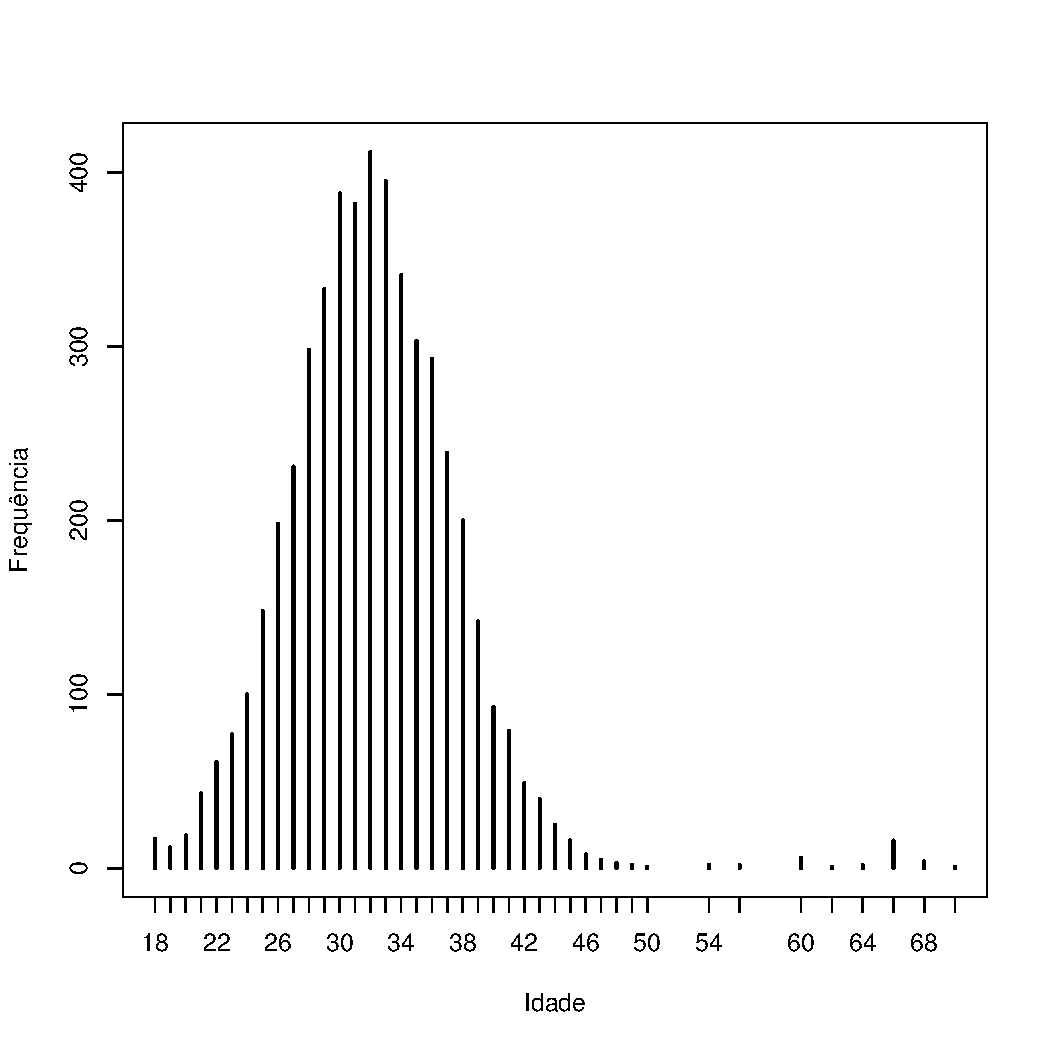
\includegraphics[width=\linewidth]{plots/histograma-idade}
	\caption{Histograma da variável idade. }
	\label{figure: histograma idade}
\end{minipage}
\end{figure}

\section*{Parte 3: Análise em Conjunto de Duas Variáveis}

\paragraph{Questão 09}

A Tabela \ref{table:satisfacao-regiao} apresenta a satisfação por região na avaliação antiga e na amostra atual. Para análise da variável \textit{Opinião} agrupada por \textit{Região}, registros com valores faltantes em qualquer uma das duas variáveis foram desconsiderados. Identificando as opiniões que compõem mais de 50\% da amostra para cada região, conclui-se que o perfil atual difere-se do antigo. Para as regiões \jaqu e \para, observou-se que a avaliação dos alunos piorou. Já para as demais regiões, percebeu-se uma melhoria na avaliação. 

Vale ressaltar que na avaliação atual, $55,29\%$ dos alunos estão satisfeitos ou muito satisfeitos. No entanto, os \textit{campi} que concentram as maiores taxas de insatisfação (\arat e \para) contém apenas $26,12\%$ dos alunos. Adicionalmente \baep, que onde os alunos estão majoritariamente satisfeitos ou muito satisfeitos, concentra $45,88\%$ dos 5000 alunos. O gráfico da Figura \ref{fig:stacked-opiniao-por-regiao} mostra visualmente como \baep e \itam mascaram o péssimo resultado de \arat e \para quando a amostra inteira é considerada.

\begin{table}[!h]
	\centering
	\caption{Satisfação por região.}
	\vspace{0.5em}
	\label{table:satisfacao-regiao}
	\begin{tabular}{l l l}
		\toprule
		\textbf{Região} & \textbf{Avaliação Antiga} & \textbf{Avaliação Atual}                \\
		\midrule
		\arat  & Muito Insatisfeito & Indiferente ($38,48\%$) e Insatisfeito ($32,15\%$)      \\
		\baep  & Muito Insatisfeito & Satisfeito ($33,96\%$) e Muito Satisfeito ($38,19\%$)   \\
		\itam  & Satisfeito         & Muito Satisfeito ($93,94\%$)                            \\
		\jaqu  & Indiferentes       & Insatisfeito ($33,93\%$) e Muito Insatisfeito ($44,03\%$) \\
		\para  & Diversas           & Muito Insatisfeito ($91,74\%$)                          \\
		\bottomrule
	\end{tabular}
\end{table}

\begin{figure}[!h]
	\centering
	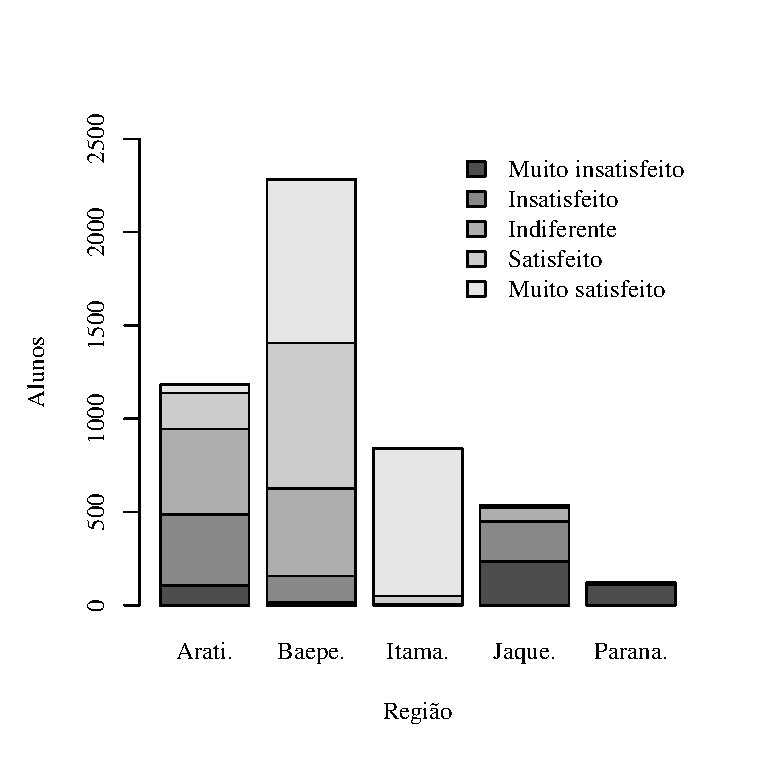
\includegraphics[width=.75\linewidth]{plots/stacked_opiniao_por_regiao.eps}
	\caption{Gráfico empilhado de opinião para cada região.}
	\label{fig:stacked-opiniao-por-regiao}
\end{figure}

\FloatBarrier
\paragraph{Questão 10}

De um modo geral, o investimento resultou em uma melhora da avaliação dos cursos \edu, \hum e \eng, e estabilidade na avaliação para os cursos de \comp e \adm. Portanto, o investimento foi eficaz. A Tabela \ref{table:opiniao-por-area} mostra a distribuição da opinião dos alunos para cada área do conhecimento, e a Figura \ref{fig:stacked-opiniao-por-area} mostra os mesmos dados usando valores absolutos de alunos em um gráfico empilhado. Tanto na Figura quanto na tabela, amostras sem valor para a variável \textit{Opinião} ou para a variável \textit{Área} foram desconsiderados no cálculo do percentual. Para análise da variáve \textit{Opinião} agrupada por \textit{Área}, registros com valores faltantes em qualquer uma das duas variáveis foram desconsiderados.

Na avaliação antiga  os cursos das áreas \edu e de \hum estavam muito insatisfeitos. Atualmente $89.91\%$ dos alunos da área \edu estão muito satisfeitos e $74.9\%$ dos alunos de \hum estão muitos satisfeitos. Considerando além de muito satisfeitos, os alunos satisfeitos, esses alunos correspondem a $97.63\%$ dos cursos da área \edu e a $91.63\%$ da área \hum.

Na avaliação antiga os cursos de \comp e de \adm elogiavam seus cursos, atualmente essa característica se mantêm. Para os cursos de \comp e os cursos de \adm, $75,26\%$ e $85.09\%$ dos alunos reportaram estarem satisfeitos ou muito satisfeitos, respectivamente.

Na avaliação antiga os alunos de cursos das demais áreas (\eng e \jur) eram tinham opinião majoritariamente indiferente. Atualmente, essa característica foi alterada. Nos cursos de \eng a quantidade de pessoas satisfeitas ou muito satisfeitas corresponde a um total de $53.82\%$, enquanto o percentual de alunos indiferentes é de $27.89\%$, indicando uma melhora. Já para o curso de Jurídica e Contábil, o percentual de alunos insatisfeitos ou muito insatisfeitos é alta, correspondendo a um total de $56.62\%$ do total de alunos, com $23.65\%$ indiferentes e apenas $19.74\%$ satisfeitos ou muito satisfeitos. Os cursos da área  \jur apresentaram uma deterioração no período e devem receber atenção especial. A urgência da tomada de ações para melhorar a opinião dos alunos da área \jur é agravada pelo grande número de alunos nessa área, correspondendo a  $30.18\%$ dos 5000 alunos na amostra.

\begin{table}[!h]
	\centering
	\vspace{0.5em}
	\caption{Opinião por área do conhecimento}
	\label{table:opiniao-por-area}
	\begin{tabular}{l r r r r r}
		\toprule
		Curso                   & \specialcell{c}{Muito\\Insatisfeito} & Insatisfeito &  Indiferente &  Satisfeito & \specialcell{c}{Muito\\Satisfeito} \\
		\midrule
		%                        Muito Ins  & Insatisfeito  & Indiferente & Satisfeito & Muito Satis           
		Administração           & $0.34\%$   & $3.57\%$     & $11.04\%$   & $28.69\%$  & $56.37\%$  \\
		Computação e Matemática & $0.68\%$   & $5.08\%$     & $18.98\%$   & $30.85\%$  & $44.41\%$  \\
		Educacional             & $0\%$      & $0.59\%$     & $1.78\%$    & $7.72\%$   & $89.91\%$  \\
		Engenharia e Produção   & $3.93\%$   & $14.26\%$    & $27.89\%$   & $26.67\%$  & $27.25\%$  \\
		Humanidades             & $0\%$      & $1.59\%$     & $6.77\%$    & $16.73\%$  & $74.90\%$  \\
		Jurídica e Contábil     & $26.45\%$ & $30.17\%$    & $23.65\%$   & $13.29\%$  & $6.45\%$   \\
		\bottomrule
	\end{tabular}
\end{table}

\begin{figure}[!h]
	\centering
	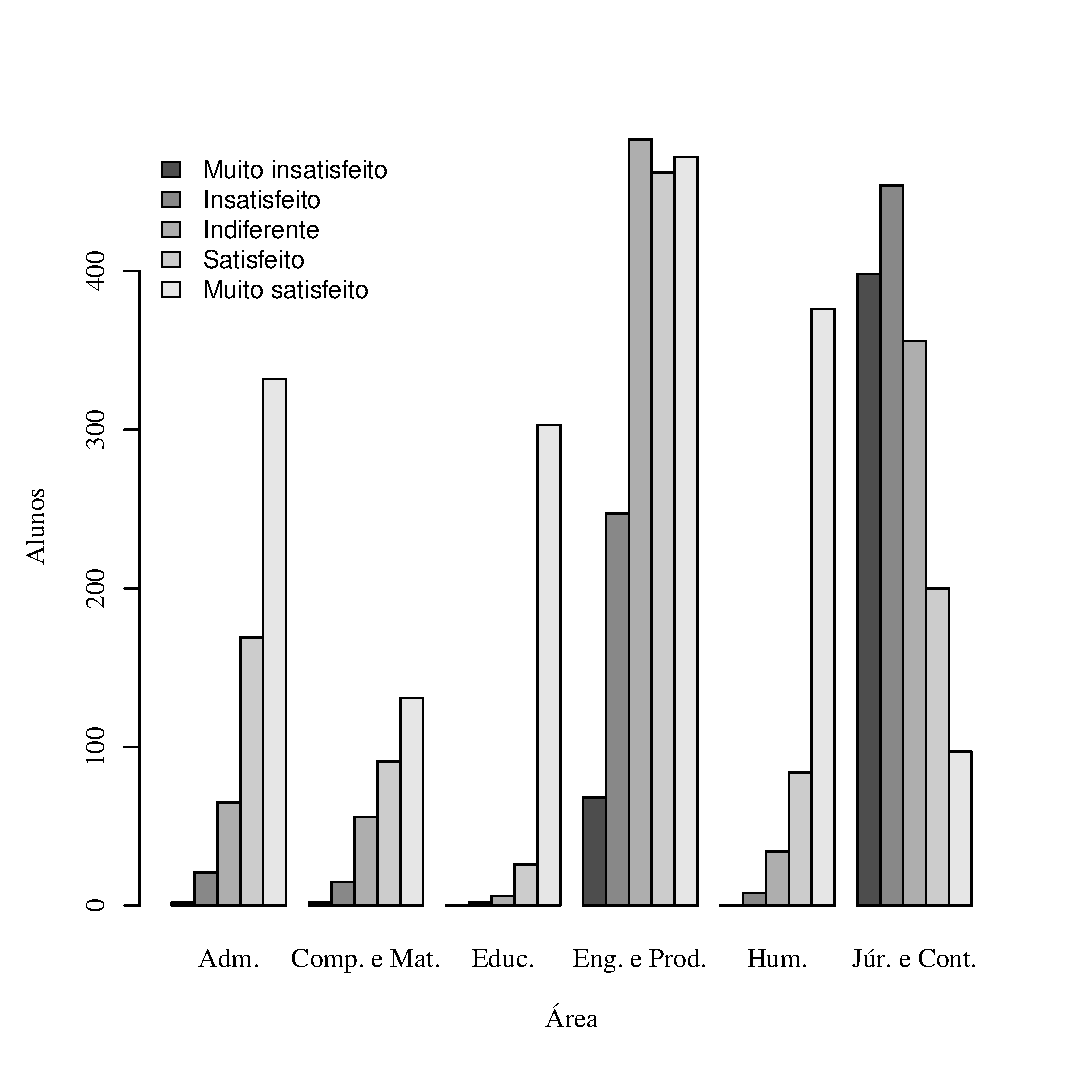
\includegraphics[width=.8\linewidth]{plots/stacked_opiniao_por_area.eps}
	\caption{Gráfico empilhado de opinião dos alunos por área do curso.}
	\label{fig:stacked-opiniao-por-area}
\end{figure}

\FloatBarrier
\paragraph{Questão 11}

As fontes de pagamento para cada uma das regiões são apresentadas em termos absolutos e percentuais na Tabela \ref{tabela: fontes de pagamento absoluto} e na Tabela \ref{tabela: fontes de pagamento percentual}, respectivamente. Adicionalmente, dados da Tabela \ref{tabela: fontes de pagamento percentual} são apresentados em formato gráfico na Figura \ref{figure: fonte de pagemento}. A composição da amostra por fonte de pagamento por região, levando em conta o número de alunos em cada região pode ser visualizado na Figura \ref{fig:fonte de pagamento absoluto}. Para análise da variável \textit{Pagamento} agrupada por \textit{Região}, registros com valores faltantes em qualquer uma das duas variáveis foram desconsiderados.

Tanto para a região \baep quanto as demais, pode-se constar uma mudança na composição da fonte de recursos para pagamentos em relação à pesquisa anterior. Para a região \baep, a nova principal fonte de recursos é oriunda de \textit{Financiamento Bancário} ($53,01\%$). Em contraste com a pesquisa anterior, \textit{Incentivos Federais} agora compõem apenas $15,08\%$ dos recursos. Para as regiões \itam, \jaqu e \para, observa-se a predominância de uma única fonte de pagamento, sendo para primeira região \textit{Financiamento Bancário}, e para as demais \textit{Incentivos Federais}. Por fim, para a região \arat, observa-se uma maior participação, mas não majoritária, de \textit{Incentivos Federais} na fonte de recursos ($47,51\%$). Cabe ressaltar que \arat e \baep apresentam composições similares para os recursos de pagamentos, mas com fontes predominantes distintas.

\begin{table}[!h]
\small
\caption{Fontes de pagamento para regiões em valores absolutos.}
\label{tabela: fontes de pagamento absoluto}
\vspace{0.5em}
\begin{tabular}{l r r r r r}
	\toprule
	\textbf{Fonte Pagamento}     & \textbf{\arat}     & \textbf{\baep}   & \textbf{\itam}  & \textbf{\jaqu} & \textbf{\para}  \\
	\midrule
	Auxílio de Familiares  & $97$       & $131$  & $10$   & $17$  & $1$    \\
	Bolsas de Estudo       & $116$      & $159$  & $7$    & $43$  & $2$    \\
	Financiamento Bancário & $180$      & $1216$ & $767$  & $20$  & $0$    \\
	Incentivos Federais    & $563$      & $346$  & $3$    & $411$ & $116$  \\
	Recursos Próprios      & $226$      & $433$  & $53$   & $43$  & $1$    \\
	\bottomrule
\end{tabular}
\end{table}

\begin{table}[!h]
\small
\caption{Fontes de pagamento para regiões em valores percentuais.}
\label{tabela: fontes de pagamento percentual}
\vspace{0.5em}
\begin{tabular}{l r r r r r}
	\toprule
	\textbf{Fonte Pagamento} & \textbf{\arat}     & \textbf{\baep}   & \textbf{\itam}   & \textbf{\jaqu} & \textbf{\para}  \\
	\midrule
	Auxílio de Familiares       & $8,19\%$           & $5,71\%$         & $1,19\%$         & $3,17\%$       & $0,83\%$  \\
	Bolsas de Estudo            & $9,79\%$           & $6,93\%$         & $0,83\%$         & $8,02\%$       & $1,65\%$  \\
	Financiamento Bancário      & $15,19\%$          & $53,01\%$        & $90,98\%$        & $3,73\%$       & $0,0\%$   \\
	Incentivos Federais         & $47,51\%$          & $15,08\%$        & $0,36\%$         & $76,68\%$      & $95,87\%$ \\
	Recursos Próprios           & $19,07\%$          & $18,88\%$        & $6,29\%$         & $8,02\%$       & $0,83\%$  \\
	\bottomrule
\end{tabular}
\end{table}

\begin{figure}[!h]
	\centering
	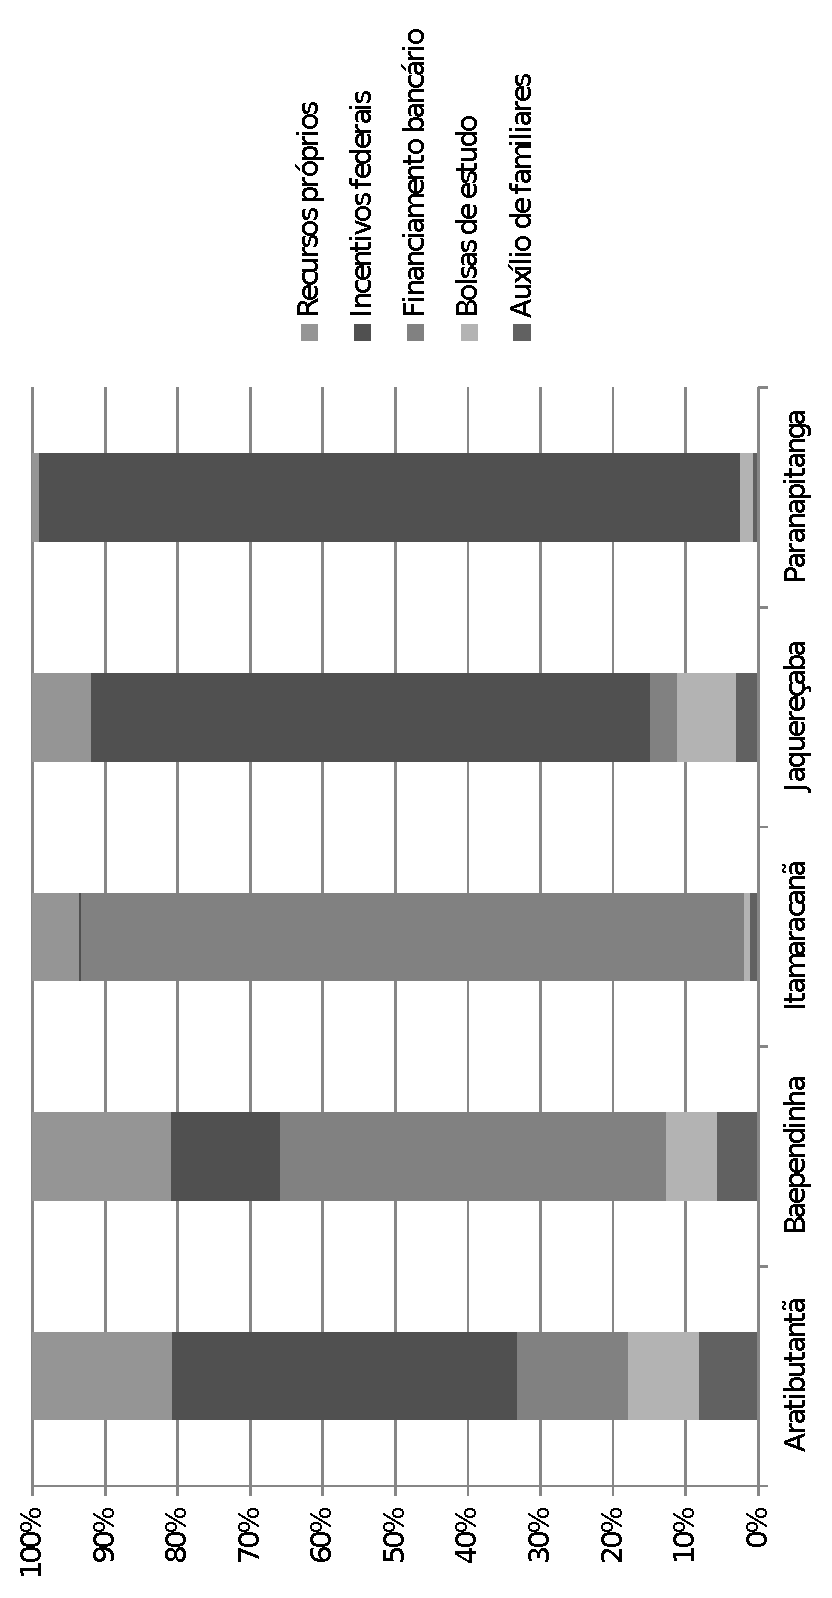
\includegraphics[width=0.80\linewidth]{plots/q11}
	\caption{Fontes de pagamento, em percentual, por região.}
	\label{figure: fonte de pagemento}
\end{figure}

\begin{figure}[!h]
	\centering
	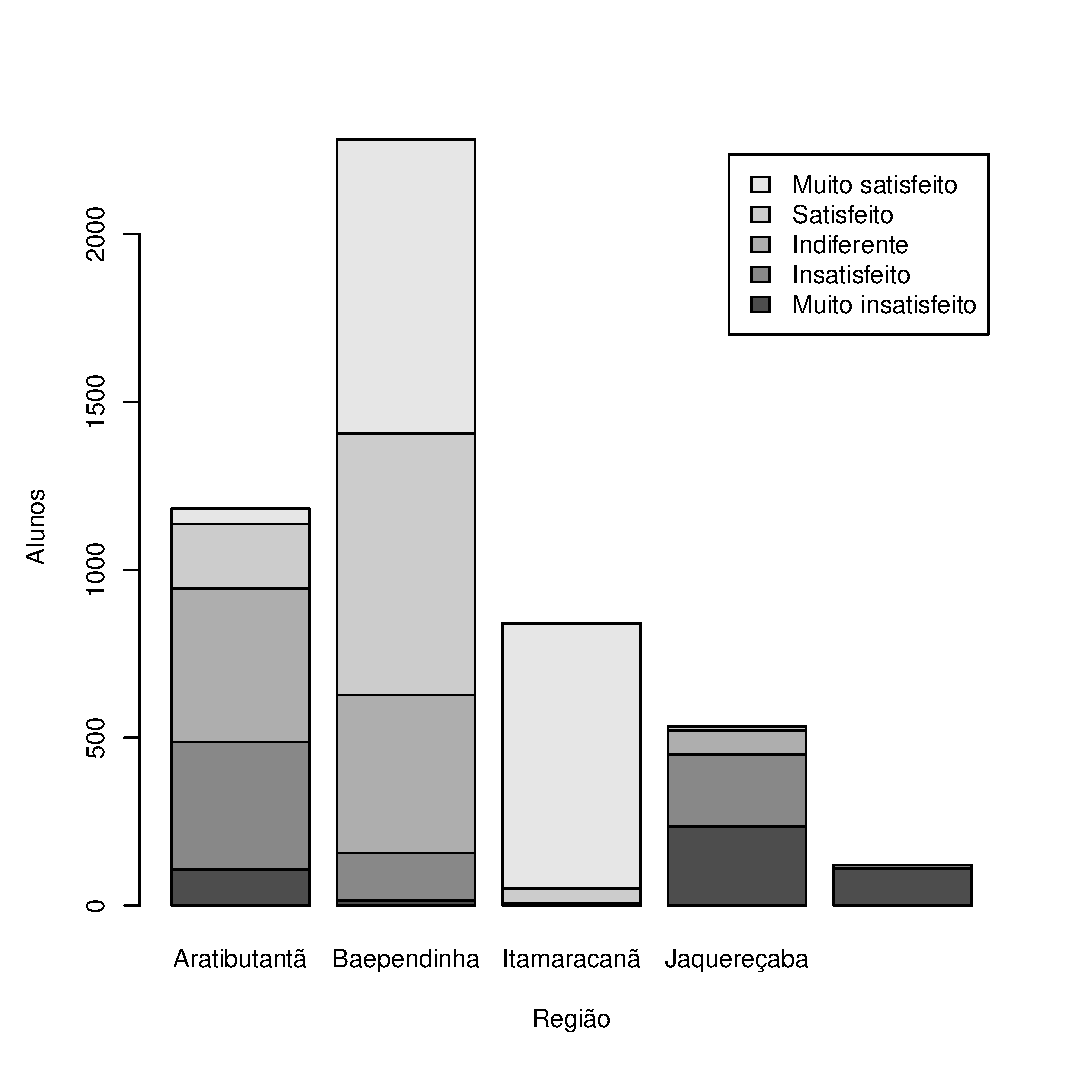
\includegraphics[width=.65\linewidth]{plots/stacked_pagamento_por_regiao.eps}
	\caption{Número de alunos por fonte de pagamento por região}
	\label{fig:fonte de pagamento absoluto}
\end{figure}

\FloatBarrier
\paragraph{Questão 12}

A avaliação dos alunos de acordo com a fonte dos recursos para pagamento é mostrada, em valores absolutos na Tabela \ref{table: avaliacao por fonte de pagamento}, e em valores relativos ao número de alunos utilizando determinada fonte, na Tabela \ref{table: avaliacao por fonte de pagamento-percent}. A Figura \ref{figure: avaliacao por fonte de pagamento} mostra os mesmos dados da Tabela \ref{table: avaliacao por fonte de pagamento-percent} na forma de um gráfico de barras empilhado. Para análise da variável \textit{Opinião} agrupada por \textit{Pagamento} foram ignorados registros com valores indisponíveis em qualquer uma das variáveis. 

As fontes de recursos podem ser divididas em duas categorias, uma onde o aluno efetivamente paga pelas mensalidades, e outra onde o o aluno não paga. O primeiro grupo é composto por \textit{Financiamento Bancário} e \textit{Recursos próprios}, enquanto o segundo é composto por \textit{Auxílio de Familiares}, \textit{Bolsas de Estudo} e \textit{Incentivos Federais}. Os resultados dessa agregação são exibidos na Tabela \ref{table:pagantes-absoluto} em valores absolutos e percentuais.

A suspeita da direção da TYU de que os alunos que recebem auxílio financeiro de alguém não são tão críticos da EAD quanto os demais, não se confirma. O grupo de alunos pagantes possui avaliações significativamente melhores de seus cursos, com $83.75\%$ dos alunos avaliando os cursos como \textit{Satisfatório} ou \textit{Muito Satisfatório}. Já entre os alunos não-pagantes, apenas $18.29\%$ se declaram \textit{Satisfeitos} ou \textit{Muito Satisfeitos}, enquanto $53.26\%$ dos alunos se declararam \textit{Muito Insatisfeitos} ou \textit{Insatisfeitos} e $36.96\%$ se declaram indiferentes. Os alunos não-pagantes são, na verdade, o grupo de alunos mais críticos ao EAD da TYU.

\begin{figure}
	\centering
	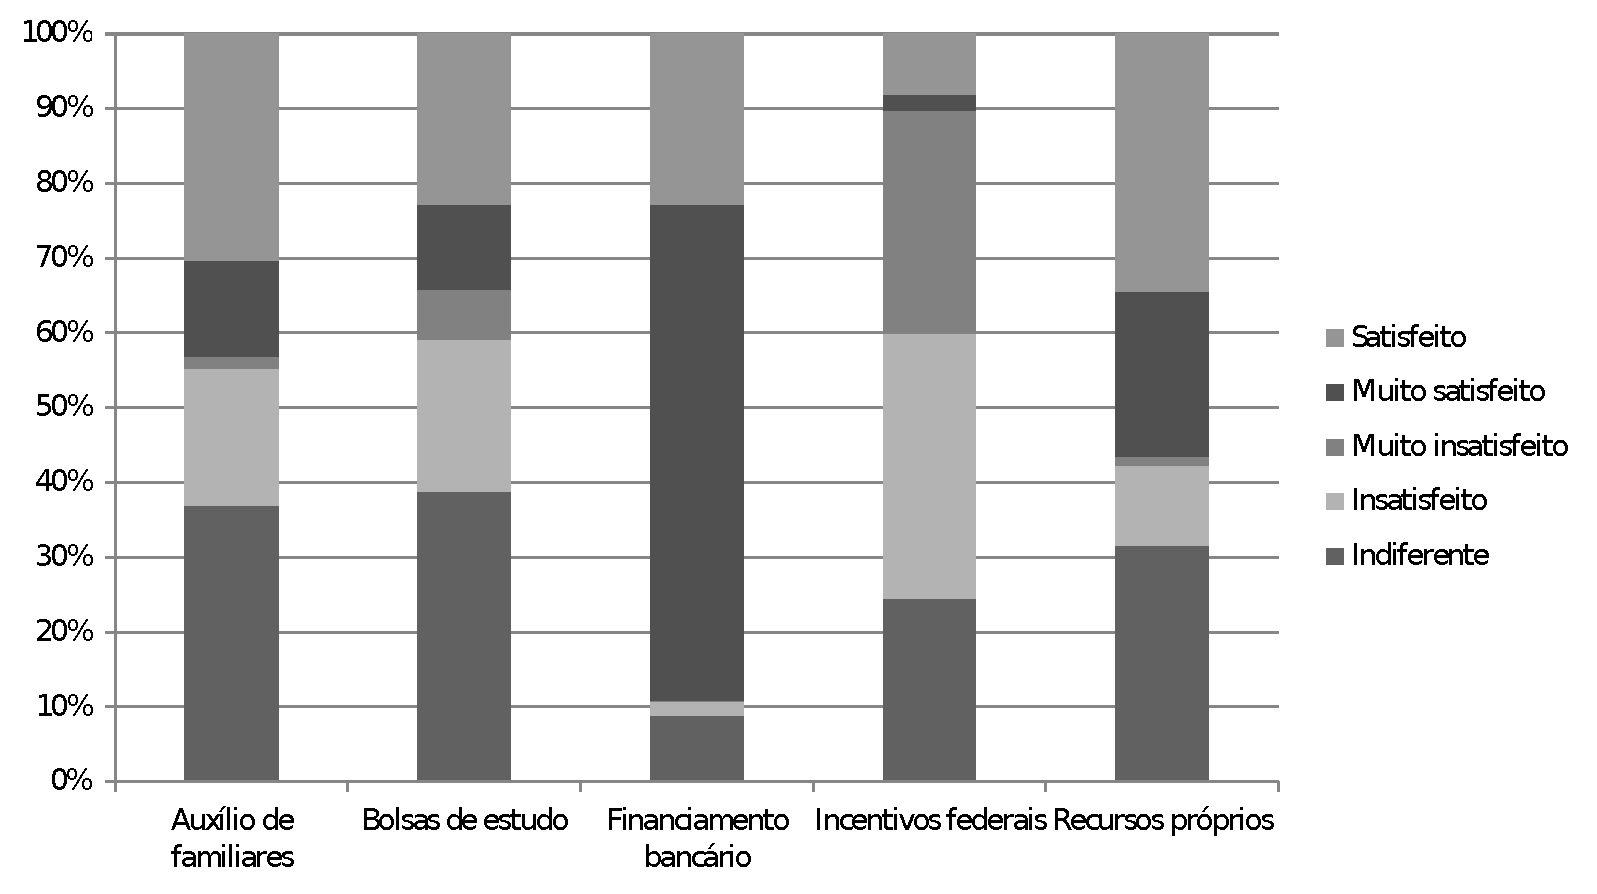
\includegraphics[width=0.80\linewidth]{plots/q12}
	\caption{Avaliação dos alunos pela fonte de pagamento}
	\label{figure: avaliacao por fonte de pagamento}
\end{figure}

\begin{table}
\footnotesize
\centering
\caption{Avaliação dos alunos pela fonte de pagamento.}
\label{table: avaliacao por fonte de pagamento}
\vspace{0.5em}
\begin{tabular}{l rrrrrr}
\toprule
	\textbf{\specialcell{c}{Fonte de\\Pagamento}}     & \textbf{\specialcell{c}{Muito\\insatisfeito}}    & \textbf{Insatisfeito}   & \textbf{Indiferente}  & \textbf{Satisfeito} & \textbf{\specialcell{c}{Muito\\satisfeito}} & \textbf{Total} \\
\midrule
	Auxílio de Familiares  & $4$      & $47$   & $95$   & $78$   & $33$   &\textbf{257}\\
	Bolsas de Estudo       & $22$     & $67$   & $127$  & $75$   & $37$   &\textbf{328}\\
	Financiamento Bancário & $3$      & $42$   & $192$  & $497$  & $1448$ &\textbf{2182}\\
	Incentivos Federais    & $431$    & $509$  & $354$  & $118$  & $30$   &\textbf{1442}\\
	Recursos Próprios      & $9$      & $81$   & $238$  & $260$  & $166$  &\textbf{754}\\
\midrule
	\textbf{Total} &\textbf{466} &\textbf{746}	&\textbf{1006}	&\textbf{1028}	&\textbf{1714}	&\textbf{4963}\\
\bottomrule
\end{tabular}
\end{table}

\begin{table}
\small
\centering
\caption{Avaliação dos alunos pela fonte de pagamento. Valores percentuais\protect\footnotemark.}
\label{table: avaliacao por fonte de pagamento-percent}
\vspace{0.5em}
\begin{tabular}{l r r r r r}
	\toprule
	\textbf{\specialcell{c}{Fonte de\\Pagamento}}     & \textbf{\specialcell{c}{Muito\\insatisfeito}}     & \textbf{Insatisfeito}   & \textbf{Indiferente}  & \textbf{Satisfeito} & \textbf{\specialcell{c}{Muito\\satisfeito}}  \\
\midrule
	Auxílio de Familiares  & $1.56\%$    & $18.29\%$    & $36.96\%$   & $30.35\%$  & $12.84\%$  \\
	Bolsas de Estudo       & $6.71\%$    & $20.43\%$    & $38.72\%$   & $22.87\%$  & $11.28\%$  \\
	Financiamento Bancário & $0.14\%$    & $1.92\%$     & $8.76\%$    & $22.68\%$  & $66.09\%$  \\
	Incentivos Federais    & $29.77\%$   & $35.15\%$    & $24.45\%$   & $8.15\%$   & $2.07\%$   \\
	Recursos Próprios      & $1.19\%$    & $10.69\%$    & $31.40\%$   & $21.90\%$  & $34.30\%$  \\
\bottomrule
\end{tabular}
\end{table}

\footnotetext{Valores perdidos não são apresentados, mas são contabilizados no cálculo da porcentagem.}

%           Mins ins   indif sats  Msats   Total
% Paga      12   123   430   757   1614    2936
% Não paga  457  623   576   271   100     2027

\begin{table}
\small
\centering
\caption{Números de avaliações para alunos nas categorias agrupadas de pagantes e não-pagantes}
\label{table:pagantes-absoluto}
\begin{tabular}{l c c c c c c}
	\toprule
	\textbf{Categoria}     & \textbf{\specialcell{c}{Muito\\insatisfeito}}     & \textbf{Insatisfeito}   & \textbf{Indiferente}  & \textbf{Satisfeito} & \textbf{\specialcell{c}{Muito\\satisfeito}} & \textbf{Total} \\
	\midrule
	%              & M Insatisf.     & Insatisf.       & Indif.          & Satisf.         & M Satisf.        & Total
	Pagante        & 12 ($0.40\%$)   & 123 ($4.18\%$)  & 430 ($36.96\%$) & 757 ($25.78\%$) & 1614 ($57.97\%$) & 2936 \\
	Não-pagante    & 457 ($22.54\%$) & 623 ($30.73\%$) & 576 ($36.96\%$) & 271 ($13.36\%$) & 100 ($4.93\%$)   & 2027 \\
	\textbf{Total} & 469             & 746             & 1006            & 10028           & 1714             & 4963 \\
	\bottomrule
\end{tabular}
\end{table}

%           Mins  ins   indif  sats   Msats   Total
% Paga      0.40  4.18  14.64  25.78  54.97    2936
% Não paga  22.54 30.73 28.41  13.36  4.93     2027

\FloatBarrier

\paragraph{Questão 13}

Para dividir a amostra em conjuntos de alunos pobres, com renda intermediária, e abastados foram utilizados os quartis inferior e superior. O quartil inferior foi calculado em $1.35$ salários mínimos, o que foi usado para definir todos os alunos com renda menor ou igual a $1.35$ salários como pobres. Similarmente, todos os alunos com renda superior ao quartil superior ($2.73$ salários mínimos) foram considerados como abastados. Os alunos com renda maior que $1.35$ e menor que $2.73$ foram considerados como de renda intermediária. Usando essa divisão de classes, a contagem e percentuais associados exibidos na Tabela \ref{fig:satisfaceo-renda} foram obtidos. A Figura \ref{fig:satisfacao-renda} mostra um gráfico empilhado com a distribuição das avaliações de acordo com a classe de renda. Para esta análise, registros com valores faltantes nas variáveis \textit{Opinião} ou \textit{Renda} foram desconsiderados.

Observando as proporções na Tabela \ref{table:satisfaca-renda}, subjetivamente, não podem ser observadas diferenças significativas entre as avaliações das classes. O perfil dos alunos mais abastados se modificou de majoritariamente indiferente para majoritariamente ($54.8\%$) \textit{Satisfeito} ou \textit{Muito Satisfeito}. O perfil dos alunos com renda intermediária se modificou de majoritariamente insatisfeitos para majoritariamente ($55.30\%$) \textit{Satisfeitos} ou \textit{Muito Satisfeitos}. Finalmente, o perfil dos alunos pobres se modificou de majoritariamente satisfeitos para majoritariamente ($55.5\%$) \textit{satisfeitos} ou \textit{muito satisfeitos}.

\begin{table}[h]
\centering
\small
\caption{Satisfação alunos de acordo com classes de renda.}
\label{table:satisfaca-renda}
\begin{tabular}{l r r r r r r}
\toprule
\textbf{Classe} & \textbf{\specialcell{c}{Muito\\insatisfeito}}     & \textbf{Insatisfeito}   & \textbf{Indiferente}  & \textbf{Satisfeito} & \textbf{\specialcell{c}{Muito\\satisfeito}} & \textbf{Total}  \\
\midrule
%                  & M Insatsf.     & Insats.        & Indif.         & Satisf.        & Muito Satisf.  & Total         \\ 
	Pobres         & 130 ($10.4\%$) & 178 ($14.2\%$) & 256 ($20.4\%$) & 260 ($20.8\%$) & 428 ($34.2\%$) & \textbf{1248} \\
	Intermediário  & 234 ($9.5\%$)  & 369 ($14.9\%$) & 502 ($20.3\%$) & 498 ($20.1\%$) & 872 ($35.2\%$) & \textbf{2475} \\
 	Abastados      & 108 ($8.7\%$)  & 202 ($16.2\%$) & 245 ($19.6\%$) & 276 ($22.1\%$) & 417 ($33.4\%$) & \textbf{1248} \\
\midrule
\textbf{Total}     & \textbf{472}   & \textbf{749}   & \textbf{1003}  & \textbf{1034}  &\textbf{1717}   & \textbf{4975} \\
\bottomrule
\end{tabular}
\end{table}

\begin{figure}[!h]
	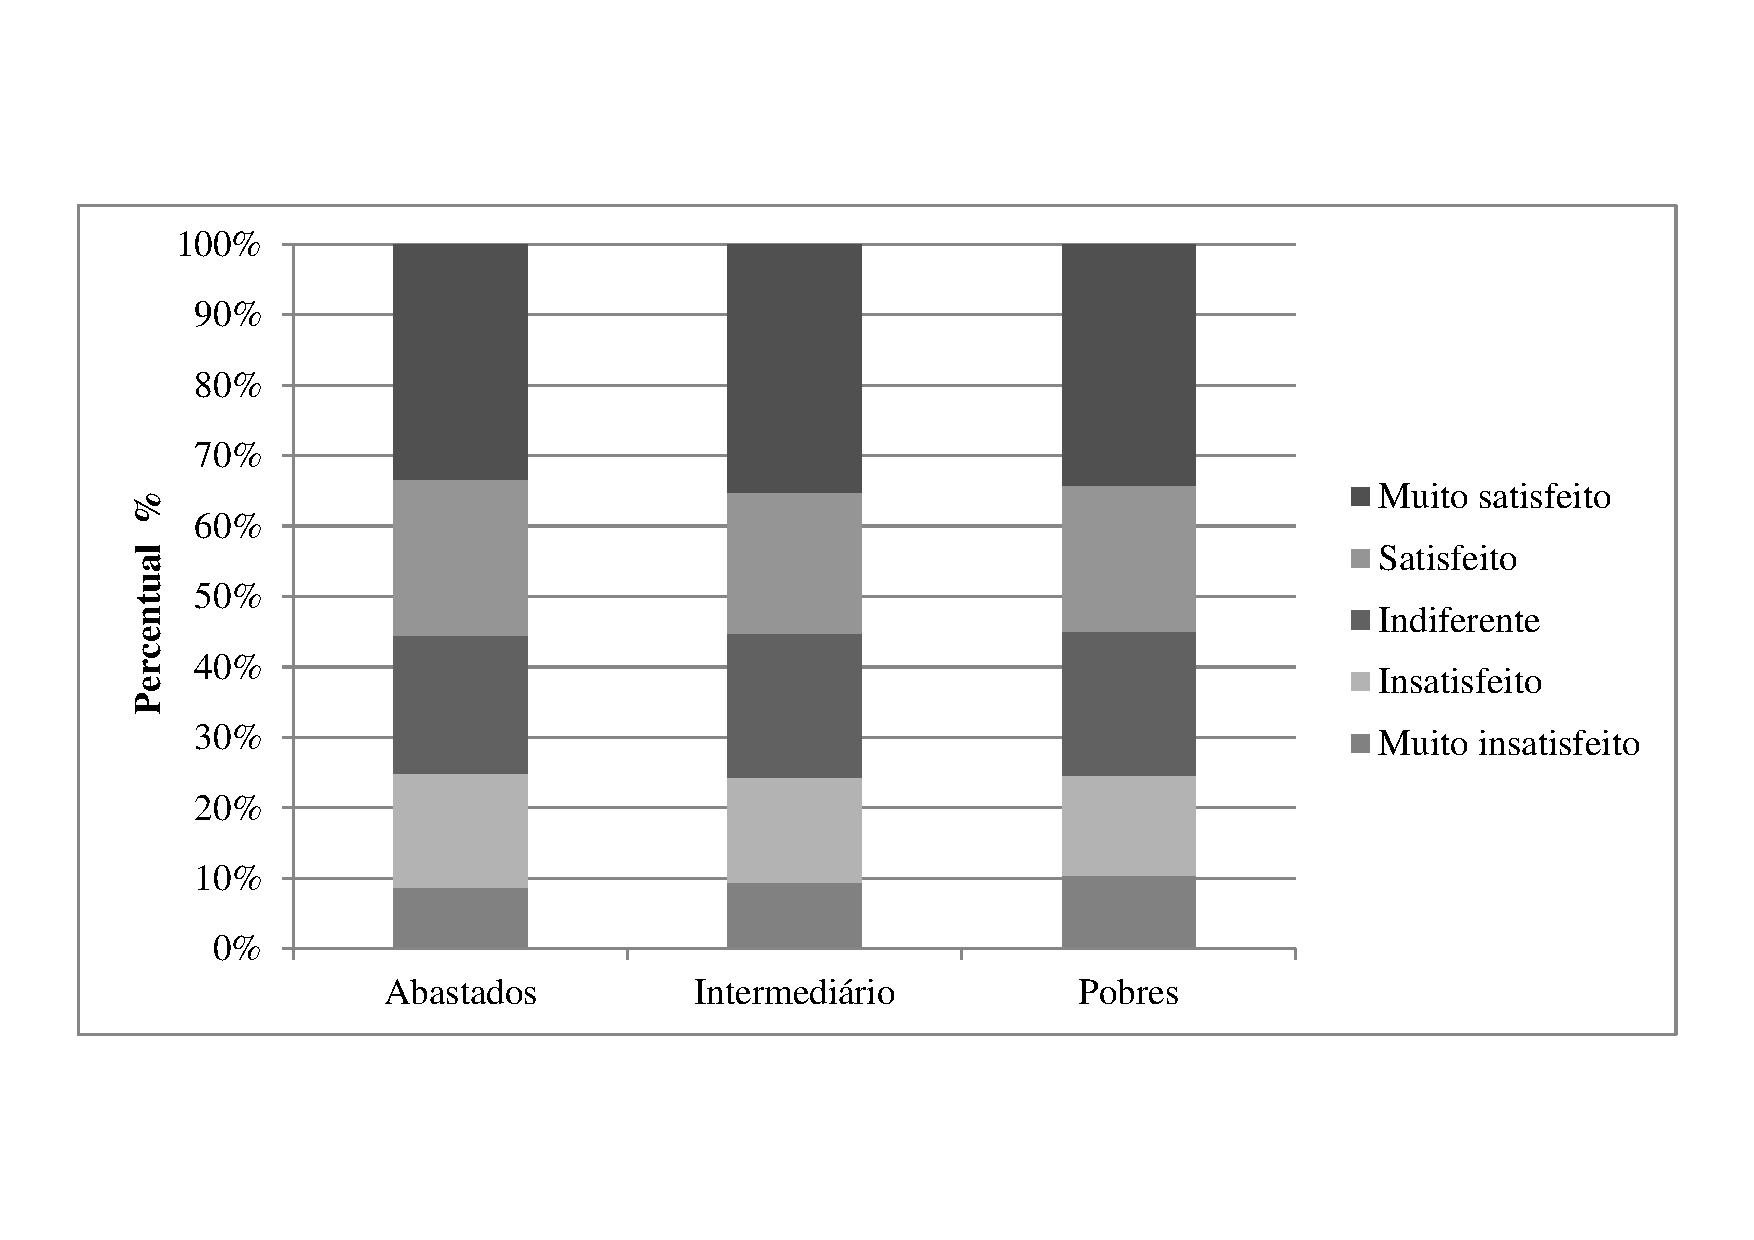
\includegraphics[width=\linewidth]{plots/q13.pdf}
	\caption{Satisfação dos alunos de acordo com classes de renda.}
	\label{fig:satisfacao-renda}
\end{figure}

\paragraph{Questão 14}

A correlação entre alunos e velhos com grau de satisfação com seus cursos é apresentada na Tabela \ref{tabela: correlacao idade cursos absoluta} e na Tabela \ref{tabela: correlacao idade cursos percentual} em termos absolutos e percentuais, respectivamente. Além disso, a Figura \ref{fig:stacked-opiniao-por-idade} sintetiza de forma gráfica os valores apresentados na Tabela  \ref{tabela: correlacao idade cursos absoluta}.

Em contraste com 10 anos atrás, quando o EAD iniciou suas atividades, no estudo atual, percebe-se uma inversão da avaliação dos alunos velhos e jovens quanto ao  seus cursos. A maioria dos alunos jovens estão satisfeitos ou muito satisfeitos com o curso ($90,73\%$). Os alunos mais velhos apresentam uma distribuição de opiniões mais uniforme onde a opinião mais popular é a indiferença com $25.62\%$ dos alunos. Há mais alunos velhos com opiniões positivas ($39.56\%$) do que alunos com opiniões negativas ($36.82\%$), então pode-se afirmar que os alunos mais velhos ainda estão mais satisfeitos ou indiferentes com relação ao seu curso. No entanto, diferentemente de antigamente, os alunos jovens estão muito mais satisfeitos que os alunos velhos.

\begin{table}[!h]
\small
\centering
\caption{Correlação absoluta de alunos novos e velhos com grau de satisfação com seus cursos.}
\vspace{0.5em}
\label{tabela: correlacao idade cursos absoluta}
\begin{tabular}{l r r r r r r}
	\toprule
	\textbf{Alunos}	& \textbf{\specialcell{c}{Muito\\Insatisfeito}} & \textbf{Insatisfeito} & \textbf{Indiferente} & \textbf{Satisfeito} & \textbf{\specialcell{c}{Muito\\Satisfeito}} & \textbf{Total} \\
	\midrule
	%                                M Ins  & Ins    & Indif  & Satisf  & M Satisf & Total
	Alunos Jovens ($< 30$ anos)     & $5$    & $15$   & $122$  & $278$   & $1111$   & $1531$  \\
	Alunos Velhos ($\geq 30$ anos) & $467$  & $734$  & $467$  & $608$   & $757$    & $3450$  \\
	\textbf{Total}                 & $472$  & $749$  & $1006$ & $1035$  & $1719$   & $4981$  \\
	\bottomrule
\end{tabular}
\end{table}

\begin{table}[!h]
\small
\centering
\caption{Correlação percentual de alunos novos e velhos com grau de satisfação com seus cursos.}
\vspace{0.5em}
\label{tabela: correlacao idade cursos percentual}
\begin{tabular}{l r r r r r}
	\toprule
	\textbf{Alunos}                & \textbf{\specialcell{c}{Muito\\Insatisfeito}} & \textbf{Insatisfeito} & \textbf{Indiferente} & \textbf{Satisfeito} & \textbf{\specialcell{c}{Muito\\Satisfeito}} \\
	\midrule
	%                              & M Insatisf  & Insatisf   & Indif      & Satisf      &  M Satisf  \\
	Alunos Jovens ($< 30$ anos)     & $0,33\%$    & $0,98\%$   & $7,97\%$  & $18,16\%$   & $72,57\%$  \\
	Alunos Velhos ($\geq 30$ anos) & $15.54\%$   & $21,28\%$  & $25,62\%$  & $21.94\%$  & $17.62\%$  \\
	\bottomrule
\end{tabular}
\end{table}

\begin{figure}[!h]
	\centering
	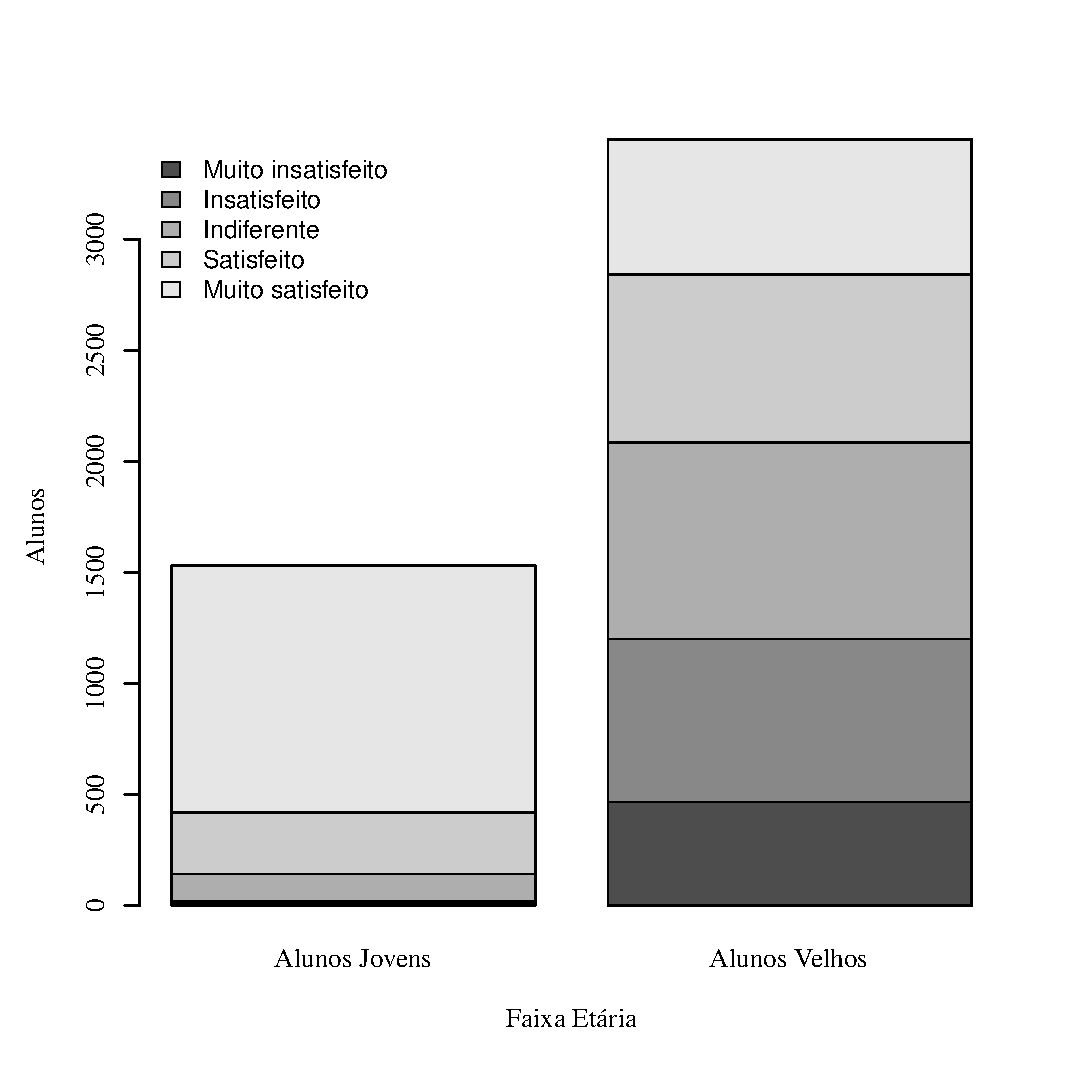
\includegraphics[width=.6\linewidth]{plots/stacked_opiniao_por_idade.eps}
	\caption{Gráfico empilhado de \textit{Opinião} por \textit{Faixa Etária}}
	\label{fig:stacked-opiniao-por-idade}
\end{figure}

\FloatBarrier
\section*{Parte 4: Análise em Conjunto de Mais de Duas Variáveis}

\paragraph{Questão 15}
Formatar tabela \ref{tabela:q15}.
% latex table generated in R 3.2.4 by xtable 1.8-2 package
% Fri Apr  8 20:51:25 2016
\begin{table}[ht]
\centering
\begin{tabular}{ll rrrrr}
  \toprule
 Área                    & Região $\vert$ Opinião & \multicolumn{1}{l}{ Muito insatisfeito} & \multicolumn{1}{l}{ Insatisfeito} & \multicolumn{1}{l}{ Indiferente} & \multicolumn{1}{l}{ Satisfeito} & \multicolumn{1}{l}{ Muito satisfeito} \\ 
   \midrule
Administração           & Aratibutantã            &                  0 &           12 &          23 &         32 &                8 \\ 
                          & Baependinha             &                  1 &            8 &          38 &        121 &              171 \\ 
                          & Itamaracanã             &                  0 &            0 &           0 &         11 &              152 \\ 
                          & Jaquereçaba             &                  1 &            1 &           4 &          2 &                0 \\ 
                          & Paranapitanga           &                  0 &            0 &           0 &          0 &                0 \\ 
\midrule
 Computação e Matemática & Aratibutantã            &                  1 &            8 &          25 &         20 &                6 \\ 
                          & Baependinha             &                  0 &            5 &          26 &         63 &               83 \\ 
                          & Itamaracanã             &                  0 &            0 &           2 &          7 &               41 \\ 
                          & Jaquereçaba             &                  1 &            2 &           3 &          1 &                0 \\ 
                          & Paranapitanga           &                  0 &            0 &           0 &          0 &                0 \\ 
\midrule
 Educacional             & Aratibutantã            &                  0 &            1 &           1 &          4 &                1 \\ 
                          & Baependinha             &                  0 &            1 &           5 &         22 &               87 \\ 
                          & Itamaracanã             &                  0 &            0 &           0 &          0 &              212 \\ 
                          & Jaquereçaba             &                  0 &            0 &           0 &          0 &                0 \\ 
                          & Paranapitanga           &                  0 &            0 &           0 &          0 &                0 \\ 
\midrule
  Engenharia e Produção   & Aratibutantã            &                 20 &          133 &         220 &         77 &               22 \\ 
                          & Baependinha             &                  5 &           44 &         224 &        356 &              300 \\ 
                          & Itamaracanã             &                  0 &            0 &           4 &         19 &              149 \\ 
                          & Jaquereçaba             &                 32 &           69 &          34 &          6 &                0 \\ 
                          & Paranapitanga           &                 10 &            1 &           0 &          0 &                0 \\ 
\midrule
  Humanidades             & Aratibutantã            &                  0 &            3 &          10 &         14 &                5 \\ 
                          & Baependinha             &                  0 &            3 &          23 &         65 &              163 \\ 
                          & Itamaracanã             &                  0 &            0 &           0 &          4 &              207 \\ 
                          & Jaquereçaba             &                  0 &            1 &           1 &          1 &                0 \\ 
                          & Paranapitanga           &                  0 &            0 &           0 &          0 &                0 \\ 
\midrule
  Jurídica e Contábil     & Aratibutantã            &                 86 &          222 &         173 &         44 &                2 \\ 
                          & Baependinha             &                  9 &           81 &         152 &        151 &               68 \\ 
                          & Itamaracanã             &                  0 &            0 &           1 &          3 &               26 \\ 
                          & Jaquereçaba             &                200 &          141 &          30 &          2 &                0 \\ 
                          & Paranapitanga           &                101 &            9 &           0 &          0 &                0 \\ 
   \bottomrule
\end{tabular}
\end{table}



\FloatBarrier
\paragraph{Questão 16}
Formatar tabela \ref{tabela:q16}.
% latex table generated in R 3.2.4 by xtable 1.8-2 package
% Fri Apr  8 21:31:49 2016
\begin{table}[ht]
\centering
\begin{tabular}{ll rrrrr}
  \toprule
 Classe        & Região $\vert$ Opinião & \multicolumn{1}{l}{ Muito insatisfeito} & \multicolumn{1}{l}{ Insatisfeito} & \multicolumn{1}{l}{ Indiferente} & \multicolumn{1}{l}{ Satisfeito} & \multicolumn{1}{l}{ Muito satisfeito} \\ 
   \midrule
Abastados     & Aratibutantã            &                101 &          263 &         127 &         16 &                1 \\ 
                & Baependinha             &                 11 &           58 &          54 &         25 &                7 \\ 
                & Itamaracanã             &                  0 &            0 &           0 &          0 &                4 \\ 
                & Jaquereçaba             &                234 &          178 &          41 &          3 &                0 \\ 
                & Paranapitanga           &                111 &           10 &           0 &          0 &                0 \\ 
  Intermediario & Aratibutantã            &                  6 &          118 &         329 &        173 &               40 \\ 
                & Baependinha             &                  4 &           84 &         411 &        670 &              450 \\ 
                & Itamaracanã             &                  0 &            0 &           6 &         30 &               76 \\ 
                & Jaquereçaba             &                  2 &           36 &          31 &          9 &                0 \\ 
                & Paranapitanga           &                  0 &            0 &           0 &          0 &                0 \\ 
  Pobres        & Aratibutantã            &                  0 &            0 &           0 &          4 &                4 \\ 
                & Baependinha             &                  0 &            0 &           5 &         84 &              419 \\ 
                & Itamaracanã             &                  0 &            0 &           1 &         14 &              710 \\ 
                & Jaquereçaba             &                  0 &            0 &           0 &          0 &                0 \\ 
                & Paranapitanga           &                  0 &            0 &           0 &          0 &                0 \\ 
   \bottomrule
\end{tabular}
\end{table}



\section*{Parte 5: Recomendações para o Cliente}

\FloatBarrier
\paragraph{Questão 17}

Para avaliar a opinião dos alunos de EAD da TYU de acordo com as variáveis \textit{Região}, \textit{Idade} e \textit{Pagamento}, pode-se construir uma tabela de frequência das opiniões relacionados aos valores filtrados das variáveis em questão. Para apresentação visual, gráficos de setores para cada conjunto de alunos são mais adequados. Conforme será detalhado a seguir para cada grupo definido no enunciado, em comparação com os dados da Tabela \ref{table:frequencias-opiniao} da \textbf{Questão 06}, o grupo \textbf{a} apresenta uma quantidade expressiva de alunos indiferentes, enquanto os grupos \textbf{b} e \textbf{c} apresentam proporções significativas de alunos insatisfeitos.

\paragraph{(a)} A Tabela \ref{table:opiniao-28anos-finBancario} apresenta as frequências dos valores de \textit{Opinião} dos alunos de \arat, com \textit{Idade} maior de 28 anos e \textit{Pagamento} do tipo \textit{Financiamento Bancário}. O gráfico de setores da Figura \ref{fig:opiniao-28anos-finBancario} mostra a porcentagem dos valores da variável \textit{Opinião} com ao menos uma ocorrência.
Pode-se observar que $41.91\%$ dos alunos são indiferentes, e que os alunos Satisfeitos e Muito Satisfeitos, juntos, somam $42.65\%$ do total de alunos. Os alunos insatisfeitos contabilizam apenas $15.44\%$ do total.


\begin{table}[!h]
	\small
	\centering
	\caption{Frequência dos valores de \textit{Opinião} para alunos de \arat com mais de 28 anos pagando mensalidade via Financiamento Bancário.}
	\label{table:opiniao-28anos-finBancario}
	\begin{tabular}{l r}
		\toprule
		\textbf{Opinião} & \textbf{Frequência} \\
		\midrule
		Insatisfeito     &  21 \\
		Indiferente      &  57 \\
		Satisfeito       &  47 \\
		Muito Satisfeito &  11 \\
		\midrule
		Total            &  136 \\
		\bottomrule
	\end{tabular}
\end{table}

\begin{figure}[!h]
	\centering
	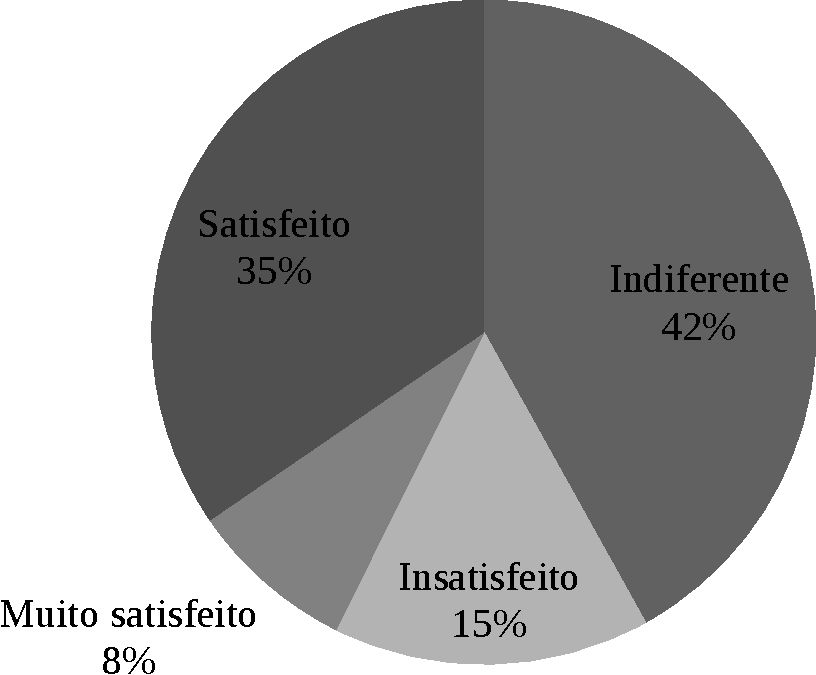
\includegraphics[width=.6\linewidth]{plots/q17a.pdf}
	\caption{Opinião dos alunos de \arat com mais de 28 anos pagando mensalidade via Financiamento Bancário.}
	\label{fig:opiniao-28anos-finBancario}
\end{figure}

\paragraph{(b)}

A Tabela \ref{table:opiniao-28anos-proprios} apresenta as frequências dos valores da variável \textit{Opinião} dos alunos que estão de \jaqu, com \textit{Idade} maior de 28 anos e Pagamento do tipo \textit{Recursos Próprios}. Os porcentuais desses valores podem ser observados no gráfico de setores da Figura \ref{fig:opiniao-28anos-proprios}.
Pode-se observar que a maioria, $53.66\%$ dos alunos, estão insatisfeitos, incluindo os alunos muito insatisfeitos, obtém-se $60.98\%$ do total. Dos $39.02\%$ restantes, a maioria é de alunos indiferentes ($34.15\%$) com apenas 2 alunos (4.88\%) se declarando satisfeitos.

\begin{table}[!h]
	\small
	\centering
	\caption{Frequência dos valores de \textit{Opinião} para alunos de \arat com mais de 28 anos pagando mensalidade via Financiamento Bancário.}
	\label{table:opiniao-28anos-proprios}
	\begin{tabular}{l r}
		\toprule
		\textbf{Opinião}    & \textbf{Frequência} \\
		\midrule
		Muito Insatisfeito  &  3  \\
		Insatisfeito        &  22 \\
		Indiferente         &  14 \\
		Satisfeito          &  2  \\
		\midrule
		Total               &  41 \\
		\bottomrule
	\end{tabular}
\end{table}

\begin{figure}[!h]
	\centering
	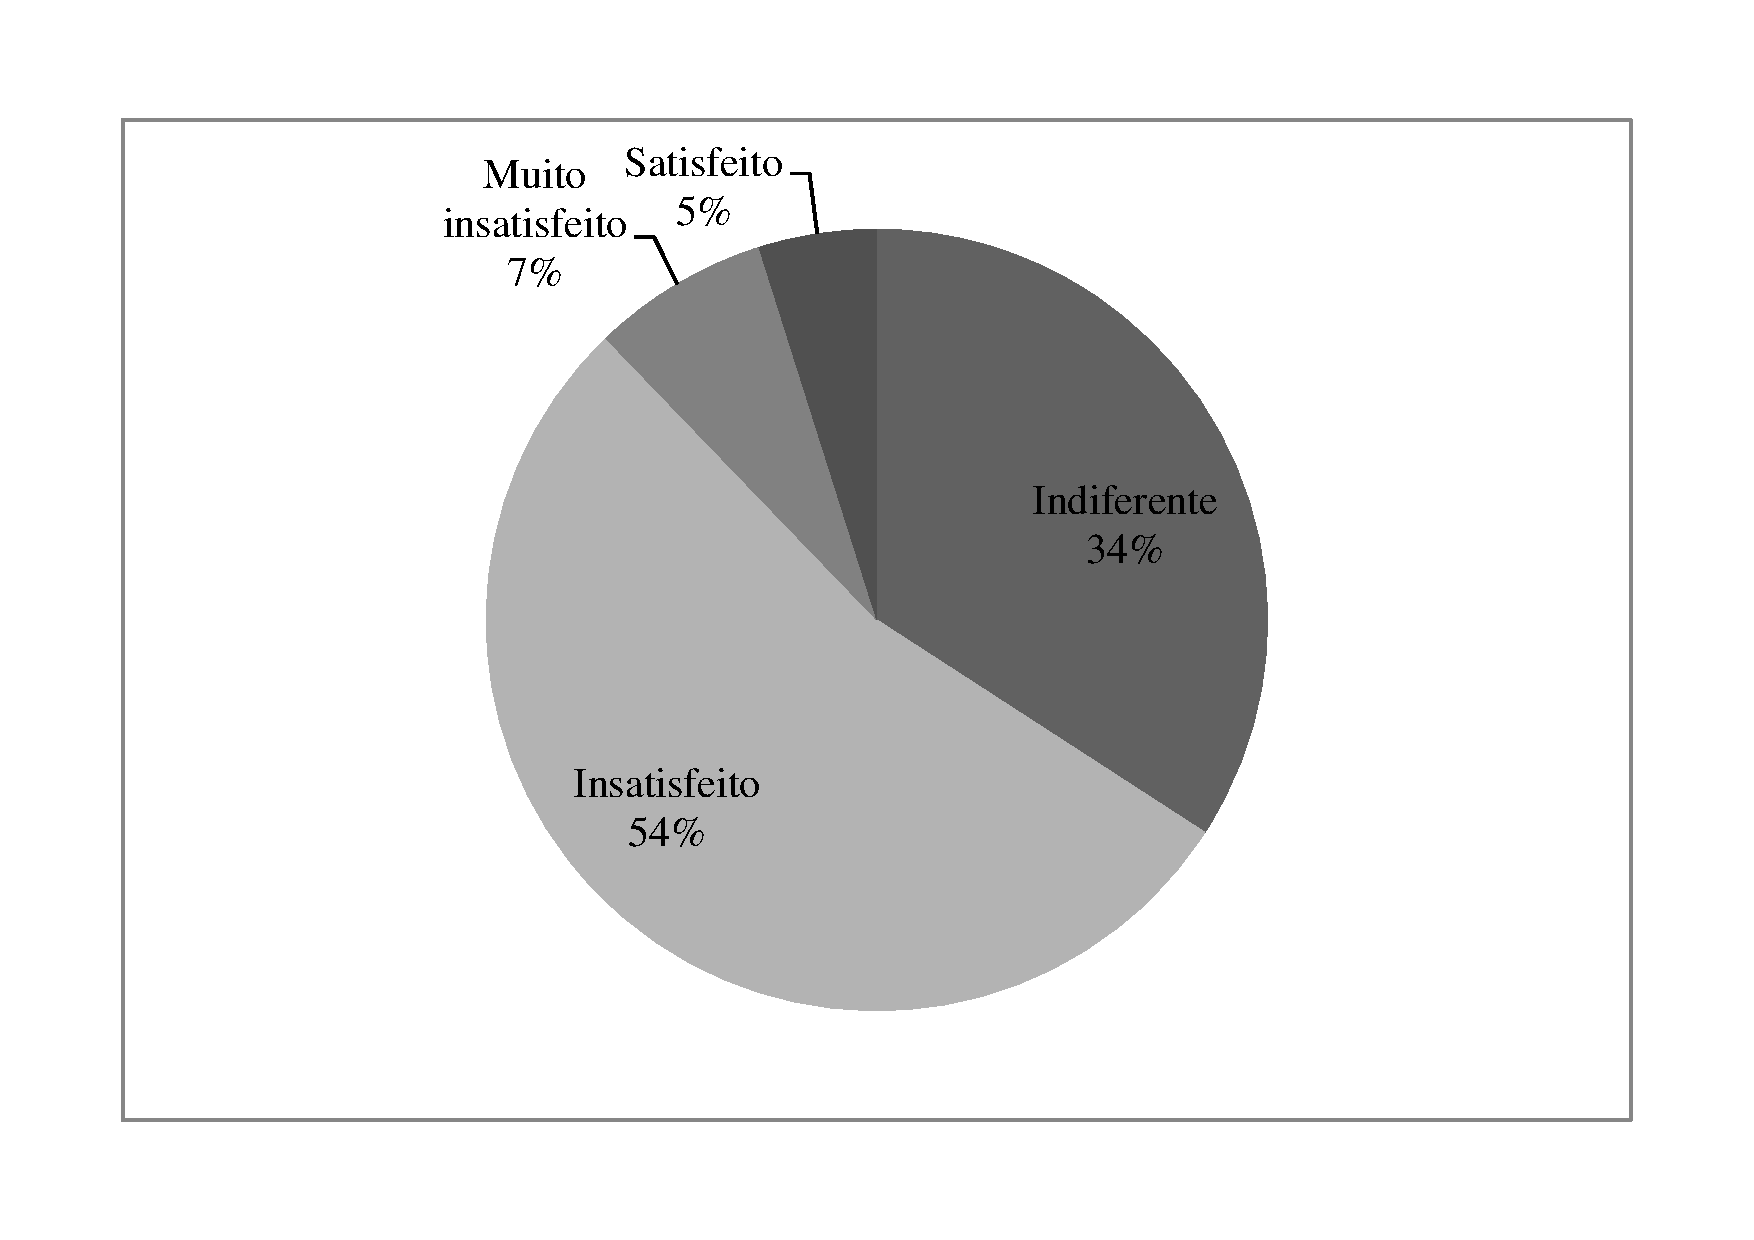
\includegraphics[width=.6\linewidth]{plots/q17b.pdf}
	\caption{Opinião dos alunos de \jaqu com mais de 28 anos pagando mensalidade com Recursos próprios.}
	\label{fig:opiniao-28anos-proprios}
\end{figure}

\paragraph{(c)}

A Tabela \ref{table:opiniao-28anos-incFederais} apresenta as frequências dos valores da variável \textit{Opinião} dentre os alunos que de \para, com mais de 28 anos e financiados por \textit{Incentivos Federais}. Uma representação desses valores é mostrada em um gráfico de setores na Figura \ref{fig:opiniao-28anos-incFederaiso}.
Pode-se observar $92.24\%$ dos alunos muito insatisfeitos e $7.76\%$ estão insatisfeitos, não havendo alunos indiferentes, satisfeitos ou insatisfeitos.
É possível notar existe uma plena insatisfação por parte alunos acima de 28 anos da região \para e que recebem Incentivos federais.

\begin{table}[!h]
	\small
	\centering
	\caption{Frequência dos valores de \textit{Opinião} para alunos de \arat com mais de 28 anos pagando mensalidade via Financiamento Bancário.}
	\label{table:opiniao-28anos-incFederais}
	\begin{tabular}{l r}
		\toprule
		\textbf{Opinião}    & \textbf{Frequência} \\
		\midrule
		Muito Insatisfeito  &  3  \\
		Insatisfeito        &  22 \\
		Indiferente         &  14 \\
		Satisfeito          &  2  \\
		\midrule
		Total               &  41 \\
		\bottomrule
	\end{tabular}
\end{table}

\begin{figure}[!h]
	\centering
	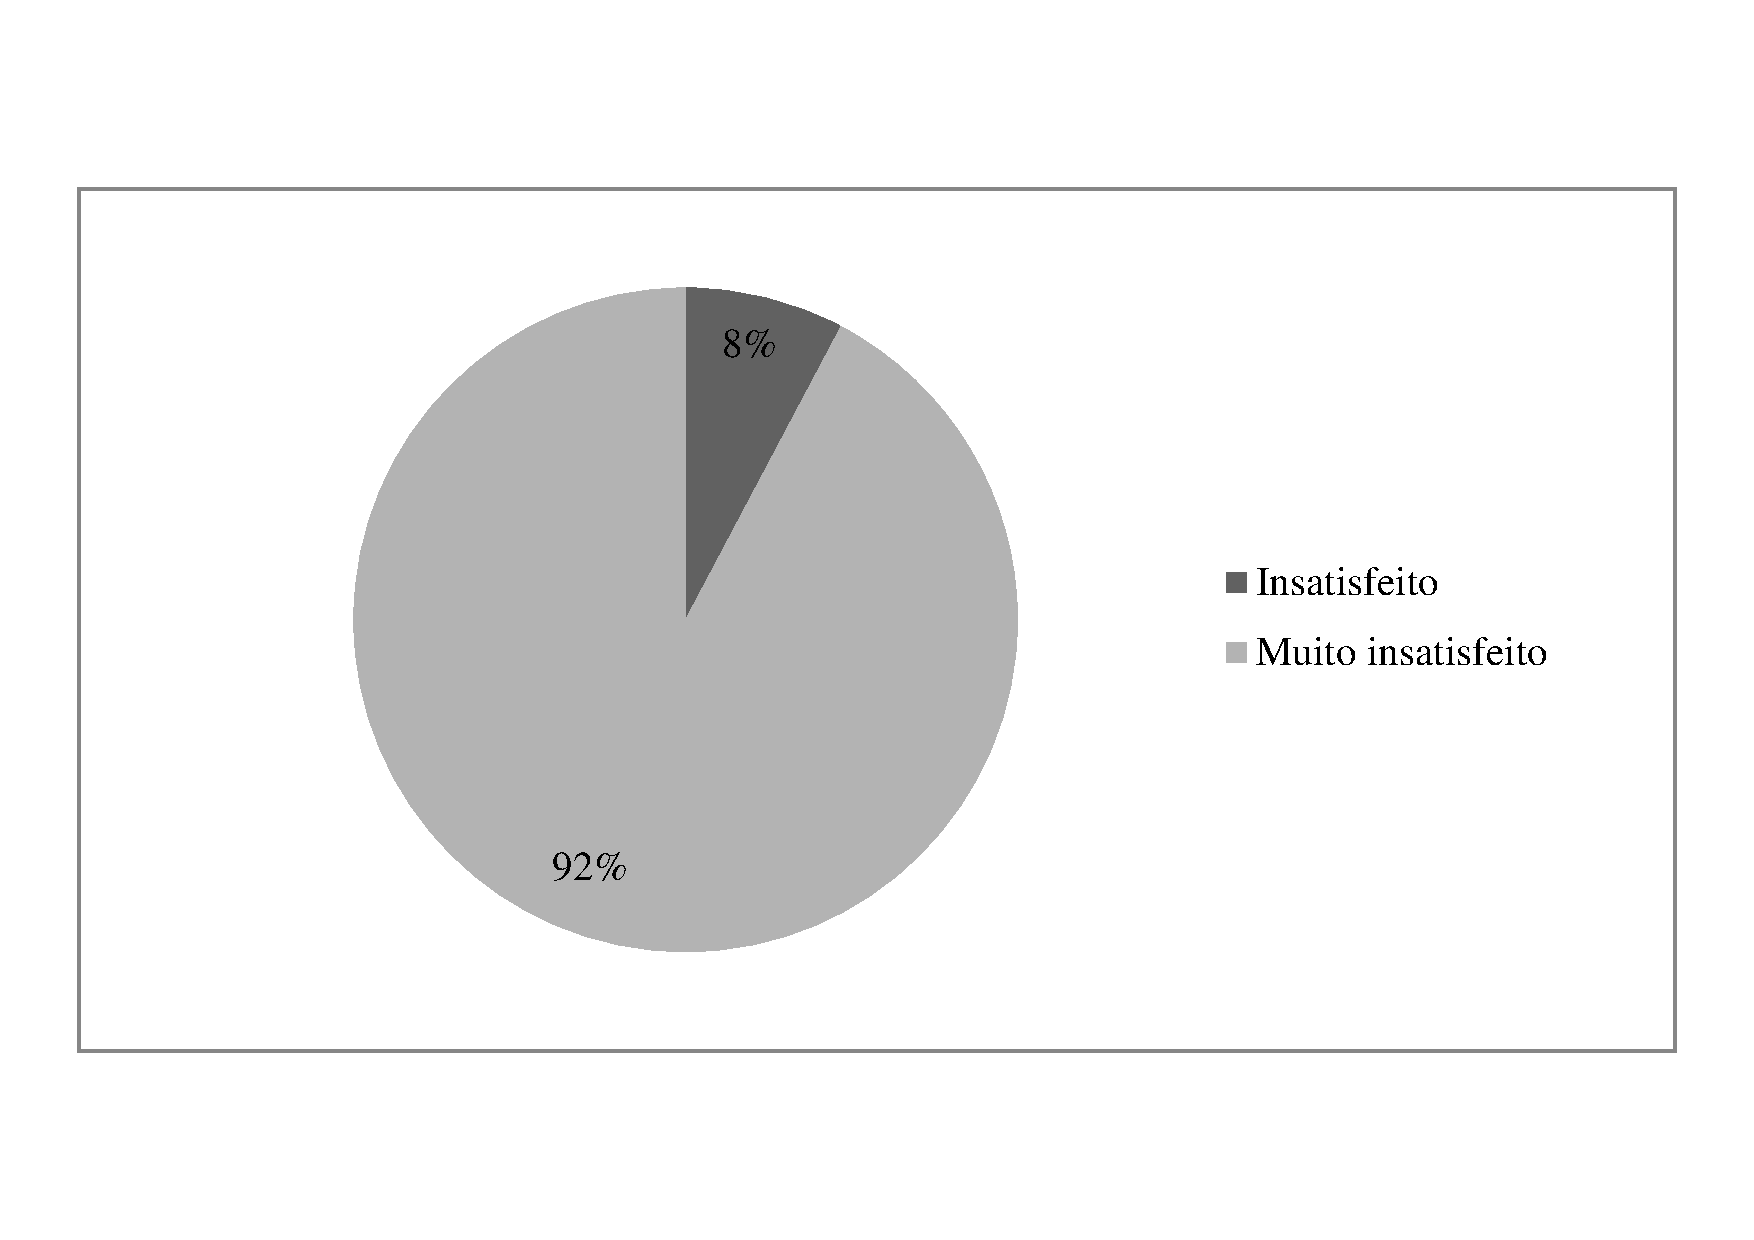
\includegraphics[width=\linewidth]{plots/q17c.pdf}
	\caption{Opinião dos alunos de \para com mais de 28 anos pagando mensalidade via Incentivos Federais.}
	\label{fig:opiniao-28anos-incFederaiso}
\end{figure}

\FloatBarrier
\paragraph{Questão 18}
Outras variáveis necessárias para caracterizar adequadamente a opinião dos alunos de EAD da TYU são  ``Gênero'' e ``Rendimento do aluno'' no curso.

% eu não concordo com algumas coisas que escrevi, não me odeiem
O Gênero tem sido uma variável popular e presente em diversos estudos disponíveis ao público. 
Amplo uso, dessa variável tem sido feito nos mais diversos contextos com objetivo de encontrar correlações entre o gênero e outras variáveis. Essa busca por correlações frequentemente pode ser associada a verificação da desigualdade de gêneros. No caso da TYU, a verificação dessa desigualdade pode motivar políticas que a reduzam, e se verificada igualdade de gênero, os resultados podem ser uados em marketing. Podem ser estudadas as seguintes relações:
\begin{itemize}
	\item Participação dos gêneros em cada região: Os alunos da TYU tem uma distribuição de gênero similar à da população da região em estudo?
	\item Participação dos gêneros por área: Como a TYU se compara nesse aspecto com outras universidades ou com os totais nacionais de Pindorama? A TYU é mais inclusiva ou ou há espaço para melhora?
	\item Distribuição da Opinião por gênero: Algum gênero está particularmente insatisfeito? Alterações podem ser estudadas para melhorar a opinião e prevenir evasão;
	\item Participação de gênero em incentivos federais e bolsas de estudo: Essas modalidades de auxílio possuem viés à um gênero?
\end{itemize}

O rendimento acadêmico do aluno pode ser usado para identificar a necessidade de mudanças na área pedagógica dos cursos e dos polos de EAD. Inclusive, nos dados analisados nesse relatório, foram incluídos apenas alunos com rendimento acadêmico superior a 5, isso é uma possível fonte de erros. Os alunos com rendimento inferior, ainda assim são alunos da TYU e a sua ausência na amostra pode ter enviesado os resultados, fazendo com que futuras ações de melhorias tomadas pela direção da TYU não levem em consideração esse grupo de alunos, possivelmente levando à uma maior evasão entre os alunos nesse grupo. Como o rendimento é uma medida particular da TYU, não é confiável realizar sua comparação com índices de outras instituições, mas assim como no caso do gênero, diversas análises em conjunto com outras variáveis são possíveis:
\begin{itemize}
	\item Qual é a distribuição do rendimento dado um dos valores de Opinião? Por exemplo, alunos insatisfeitos com rendimento alto pode ser um indicativo de ensino e avaliação pedagógica muito frouxos.
	\item Qual a distribuição do rendimento em cada área em cada região? Quais cursos em quais polos precisam de mais atenção quanto os tutores e professores? Essa análise poderia guiar o investimento em laboratórios, e contratação de tutores e docentes;
	\item Qual a distribuição do rendimento por fonte de pagamento? Alunos contemplados com Bolsas ou incentivos federais estão apresentando desempenho acadêmico superior aos seus pares que possuem outros tipos de financiamento? 
	\item Qual a distribuição do rendimento por renda? Alunos pobres conseguem manter um rendimento acadêmico similar aos demais grupos de renda? Refinando essa análise fazendo agrupamentos por fonte de pagamento seria possível identificar grupos de alunos de acordo com renda e fonte de pagamento que precisem de atenção pedagógica especial;
\end{itemize}


\end{document}
